
\documentclass[review,12pt,authoryear]{elsarticle}

%% The amssymb package provides various useful mathematical symbols
\usepackage{amssymb}
%% The amsthm package provides extended theorem environments
%% \usepackage{amsthm}

%% The lineno packages adds line numbers. Start line numbering with
%% \begin{linenumbers}, end it with \end{linenumbers}. Or switch it on
%% for the whole article with \linenumbers.
\usepackage{lineno}

% for adjusting table width automatically
\usepackage{adjustbox}
\usepackage{tabulary, ragged2e}
\usepackage{booktabs}
\usepackage{longtable}

% Below is Elseviers requirements - they are similar to most articles and a good point of reference when writting scientific articles or analyses in general.
%1.Full Length Article A full-length article should be a substantial and in-depth research study regarding a particular state of issue through several techniques or approaches. 
% The main text should be approximately 6,000 words in length, but it should not exceed 8,000 words (excluding abstract, references, tables, figures, and appendices).
%A maximum of 250 words abstract and up to 10 displayed items (figures and tables) is allowed. A full-length article should include an Introduction,
%Materials and methods, Results, Discussion, Conclusions, and References, which can be accompanied by Supplementary material.

\begin{document}
\begin{linenumbers}
\begin{frontmatter}

%%%%%%%%%%%%%%%%%%%%%%%%%%%%%%%%%%%%%%%%%%
%%       Start Matter      %%
%%%%%%%%%%%%%%%%%%%%%%%%%%%%%%%%%%%%%%%%%%

%% Title, authors and addresses

%% use the tnoteref command within \title for footnotes;
%% use the tnotetext command for theassociated footnote;
%% use the fnref command within \author or \affiliation for footnotes;
%% use the fntext command for theassociated footnote;
%% use the corref command within \author for corresponding author footnotes;
%% use the cortext command for theassociated footnote;
%% use the ead command for the email address,
%% and the form \ead[url] for the home page:

%% \title{Title\tnoteref{label1}}
\title{An analysis of underlying relationships between factors related to operating costs and revenue in Australian vineyards.}

% Variable importance in determining vineyard operational costs and region using statistical machine learning.
% How are region and operational costs related?

% Regional differences in Australian winegrowing (Quality)?

%% \tnotetext[label1]{}
%% \author{Name\corref{cor1}\fnref{label2}}
%% \ead{email address}
%% \ead[url]{home page}
%% \fntext[label2]{}
%% \cortext[cor1]{}
%% \affiliation{organization={},
%%      addressline={}, 
%%      city={},
%%      postcode={}, 
%%      state={},
%%      country={}}
%% \fntext[label3]{}

%% use optional labels to link authors explicitly to addresses:
%% \author[label1,label2]{}
%% \affiliation[label1]{organization={},
%%       addressline={},
%%       city={},
%%       postcode={},
%%       state={},
%%       country={}}
%%
%% \affiliation[label2]{organization={},
%%       addressline={},
%%       city={},
%%       postcode={},
%%       state={},
%%       country={}}
%\affiliation[label1]{organization={QUT},
% addressline={},
% city={},
% postcode={},
% state={QLD},
% country={}}
%\affiliation[label2]{organization={AWRI},
% addressline={},
% city={},
% postcode={},
% state={SA},
% country={}}
%\affiliation[label3]{organization={Food Agility CRC},
% addressline={},
% city={},
% postcode={},
% state={Vic},
% country={}}
\author[label1,label2,label3]{Author}
\date{02/08/2023}

\begin{abstract}

 The Australian wine industry is a major contributor to Australia's agricultural sector and economy. As global market demands change and new pressures on the industry present themselves, a more sustainable approach is needed. Through a nationwide data set, collected over ten years, we link key variables in determining vineyard operational costs and revenue through the use of XGBoost. We use a measure of relative importance to show the interrelated nature of these variables and the comparative influence they have on one another. We present these connections through the use of Sankey and Chord diagrams to show the important predictors of revenue and operating costs and their strong interrelatedness. Furthermore, we connect these variables to different wine regions, highlighting the complex influence of location on the use of different resources. The study provides valuable insights into the multifaceted dynamics governing operational costs and revenue, illustrating how factors such as water and fuel use impacts operational costs and how different seasonal events affect these operations. 


\end{abstract}
%%Graphical abstract`
%\begin{graphicalabstract}
 % \includegraphics{graphical_abstract.jpeg}
%\end{graphicalabstract}'

%\begin{keyword}
%% keywords here, in the form: keyword \sep keyword
%Keyword one \sep{} keyword two
%% PACS codes here, in the form: \PACS code \sep code
%\PACS{} 0000 \sep{} 1111
%% MSC codes here, in the form: \MSC code \sep code
%% or \MSC[2008] code \sep code (2000 is the default)
%\MSC{} 0000 \sep{} 1111
%\end{keyword}
%%Research highlights
% \begin{highlights}
%  \item Highlight 1
%  \item Highlight 2
%  \item Highlight 3
%  \item Highlight 4
% \end{highlights}
\end{frontmatter}

%%%%%%%%%%%%%%%%%%%%%%%%%%%%%%%%%%%%%%%%%%
%%        main text       %%
%%%%%%%%%%%%%%%%%%%%%%%%%%%%%%%%%%%%%%%

%%%%%%%%%%%%%%%%
% Working title
%

% Description
% NB Avoid titles along the lines of: “Effects of ...”, “The role of ...”, etc.  Be specific about the effect and its significance so that your reader knows what is on offer.
%  TODO:

% For example, rather than write a title like “The effect of factor X on astrophysical properties of green cheese.”, 

% be specific about the effect and write something more like ...

% “Factor X halves the lunar thermal diffusivity of  green cheese”.

% You will usually find it easier to write an effective title if you make your title a sentence.

% Notes
% N/a

\section{Introduction}

Historically strong demands for Australian wine have helped to create a thriving industry. However, recent pressures brought on by a loss of tourism and labour due to the COVID-19 pandemic, the global freight crisis, war in Europe, tariffs and rising inflation have negatively affected the industry's outlook \citep{wineaustraliaNationalVintageReport2021,wineaustraliaAustralianWineProduction2021}. The 2021-2022 financial year alone saw a decline of 19\% in exports solely due to tariffs \citep{wineaustraliaNationalVintageReport2022}. A greater understanding of the different underlying conditions leading to improved performance in agricultural productivity and sustainability at scale is key to making data-informed decisions to increase a nation's agricultural sustainability \citep{oecdInnovationProductivitySustainability2019}. Specifically within the Australian wine and vine industry, there is a need to further understand the driving relationships between resource use and economic output, which can help to determine more cost effective and efficient methods and develop benchmarks with local growers \citep{lukemanciniUnderstandingAustralianWine2020}.
\par
An unprecedented amount of data regarding the Australian winegrowing industry has been collected through the Sustainable Winegrowing Australia program, offering the potential for new insights into the driving economic forces of the Australian wine industry. A major part of the potential for insight within this dataset comes from the incorporation of operating costs and grape revenue from grape sales within the data. In this paper, we use data to study economic outcomes and their statistical relationships to vineyards' utilisation of the resources. We further compare the relationships between different resources to address the extensive collinearity found within the data \citep{chenXGBoostScalableTree2016}. We adopt  a popular, relatively new machine learning method, XGBoost, for this analysis because it is able to overcome multicollinearity as well as highlight the level of importance that predictor variables have on response variables.

\section{Methods}
% TODO:
%  From the code comments~ We might want to show the relationship between revenue and operational cost! then we have an idea of how these two are related.
% # These are artefacts of. As profit can be negative it is harder to predict! We know after some further mapping that both operational costs and gross margin have a cubic root relationships to the logarithm of other variables. An interesting relationship to have!
% # 
% # Importantly this cubic root relationship exists between operational costs and gross margin, which is worth noting. However we want to know what tips it either side of them being equal as that shows that a vineyard is profitable!!

\subsection{Data}\label{Data}
% 6049 samples - total
% 58 regions
% 10 years
% 
% 853 with reported profits
% 46 regions
% reported since 2018
Data used in this analysis were obtained from Sustainable Winegrowing Australia (SWA), Australia's national wine industry sustainability program. SWA aims to support grape growers and winemakers in demonstrating and improving their sustainability \citep{swaSustainableWingrowingAustralia2022}. Data recorded by SWA are entered manually by winegrowers using a web based interface tool. A total of 6049 observations were collected from 2012/2013 to 2021/2022 financial years, with each observation comprising 23 variables reflecting a vineyard's state for the given year (see Table \ref{tab:vars}). 
\par
\begin{table}[] 
 \label{tab:vars}
 \caption{Summary of variables used in the analysis. The recorded column indicate the number of values that were either greater than zero or that were not missing (see Appendix for more information).}\label{tab:summary}
 \small
% Please add the following required packages to your document preamble:
% \usepackage{booktabs}
\begin{table}[]
  \begin{tabular}{@{}lccc@{}}
  \toprule
  \textbf{Variable} & \textbf{Units} & \textbf{Number of Classes} & \textbf{No. Records} \\ \midrule
  Water Used & Mega Litres &  & 5846 \\
  Diesel & Litres &  & 5585 \\
  Biodiesel & Litres &  & 25 \\
  LPG & Litres &  & 958 \\
  Herbicide Spray & No. Times per year &  & 2026 \\
  Year & Class & 10 & 6049 \\
  Disease & Class & 2 & 6049 \\
  Region & Class & 58 & 6049 \\
  Solar & Kilowatt Hours &  & 622 \\
  Irrigation Type & Class & 20 & 6049 \\
  Petrol & Litres &  & 4309 \\
  Slashing & No. Times per year &  & 2290 \\
  Yield & Tonnes &  & 5935 \\
  Irrigation Energy & Class & 16 & 6049 \\
  Area Harvested & Hectares &  & 6049 \\
  Electricity & Kilowatt Hours &  & 1014 \\
  Insecticide Spray & No. Times per year &  & 1092 \\
  Fertiliser & KGs of Nitrogen &  & 795 \\
  Fungicide Spray & Times per year &  & 2260 \\
  Cover Crop & Class & 32 & 6049 \\
  Water Type/Source & Class & 39 & 6049 \\
  Grape Revenue & AUD &  & 853 \\
  Operating Costs & AUD &  & 853 \\ \bottomrule
  \end{tabular}
  \end{table}
\normalsize
The data originally contained only two multiclass variables: year and region. For this case study, related binary variables, such as the use of river water and the use of dam water, were combined to create multiclass variables such as water source/type. Further details about these variables, their classes and their frequency is available in the Appendix.
\par
The variable Region represented one of the 65 Geographical Indicator Regions (GI Region) used to describe unique localised traits of vineyards across Australia \citep{hallidayAustralianWineEncyclopedia2009,oliverReviewSoilPhysical2013,soarClimateDriversRed2008}. Each region is explicitly defined under the Wine Australia Corporation Act of 1980 \citep{attorney-generalsdepartmentWineAustraliaCorporation2010}.
\par

\subsection{XGBoost}
XGBoost (eXtreme Gradient Boosting), described in more detail below (and further in the Appendix), were created using the XGBoost library \citep{chenXGBoostScalableTree2016} in the Python Programming language \citep{g.vanrossumPythonTutorialTechnical1995}. XGBoost is a type of machine learning method that constructs and ensemble of decision trees to predict or estimate an output variable (the response) based on a number of input variables. The ensemble, can be used to classify classes or predict a continuous response, depending on the nature of the output variable. They were chosen for this analysis as the data contained a mixture of class and continuous variables. Moreover, XGBoost is unaffected by multicollinearity, and offer high predictive performance for a wide variety of purposes, and are capable of identifying and ranking variables and interactions in order of relative importance \citep{chenXGBoostScalableTree2016}.
\par
Four sets of analyses were conducted. In the first set, two XGBoost models were developed, with operational cost and grape revenue as the response variables. The analysis of operational cost and revenue included all variables in Table \ref{tab:vars}. The second set of analyses focused on identifying relationships between the input variables themselves, creating XGBoost models for each other variable so that every variable would have a measure of its relative importance to every other variable (see Section \ref{sec:importance}). Together these models were used to measure the interrelationships of the ten most important variables in determining operational cost and grape revenue using variable importance. These measures of relative importance were used to illustrate the highly interrelated nature of variables within vineyards. The interaction between variables was depicted through the use of Sankey and Chord diagrams; with variable importance measures being used to show the strength of connection between the respective predictor variables and the response (see section \ref{sec:importance}).
\par
The third analysis was an XGBoost tree with Region as the response variable. The difference for this model was that relative variable importance for each variable would be measured for the overall importance in determining region, as opposed to a variable's connection to each region specifically. The fourth analysis focussed on profit (the difference between revenue and operational costs) and year, however these results were not included due to low average loss values and model stability (see Appendix).
\par
XGBoost is an ensemble method that combines multiple decision trees together to create a more accurate predictive model. The gradient boosting aspect of the ensemble is the use of a loss function to create new decision trees that add to the ensemble, improving its predictive power. The loss function is optimised iteratively to improve upon prior trees. The loss function can be any convex function, allowing gradient descent to traverse the loss space until no substantive improvements can be made via traversal. Because the loss function is only required to be convex, both classifiers and regressors can be used. Regularisation methods can also be incorporated to help prevent over fitting. This makes XGBoost incredibly versatile and accurate, whilst still being interpretable compared to other machine learning methods.
\subsection{Variable Importance}\label{sec:importance}
XGBoost creates a large number of decision trees in the ensemble, it is hard to directly interpret the model and the derived intricate relationship between the variables. Variable importance can be measured in multiple ways, in this paper we used the frequency of a variable appearing as a node within the ensemble as a measure of its importance. This measure can be interpreted as how often a variable was the optimal choice in reducing the loss function of the ensemble. Multiclass variables are given an importance score for each individual class;  for example, in the first set of analyses each specific region will have its own importance score, as will Year, Irrigation Type, etc (see Table \ref{tab:vars}).
\par
The Sankey and Chord diagrams were constructed using the Holoviews python library \citep{philipp_rudiger_2020_3904606}. Both Chord and Sankey diagrams illustrated variable importance through the size of the bands between two variables. The number at the end of a connection in a Sankey diagram indicates a variable's importance (the number of times it appeared within the ensemble). Sankey and Chord diagrams are presented together; with Sankey diagrams showing the connection of a variable to its ten most important predictor variables and chord diagrams showing the interconnectedness of the ten most prominent variables within its associated Sankey diagram. Chord diagrams formed circles, with variables being connected through their relative importance.

\subsection{Validation}

The predictive accuracy of each tree was assessed through a validation process. For each model, a sample of 80\% of the data was used for training the model and the remaining 20\% was used for testing and validation. Categorical data were stratified to conserve the same proportion of class occurrences between the training, testing and validation data. The models were validated using 10 repetitions of the sampling process (10-fold cross validation). $R^2$ scores were used to determine the best regression models during validation. For analyses with continuous responses $R^2$ was used instead of RMSE to allow the comparison of  models with different units to each other when considering how well each model extrapolated to further data. For binary and multiclass variables, validation was summarised through the accuracy, the proportion of true negatives and positives.
\par
As with most machine learning methods, a key component of the XGBoost model setup was the tuning of hyperparameters. The XGBoost library incorporates regularisation techniques built into the software to mitigate over-fitting and enhance model generalisation. This allowed us to utilise cross validated grid search functions when selecting for better performing hyperparameters. The performance measure for model selection was root-mean-square error for continuous variables. The receiver operator characteristic's area under the curve was used for category variables \citep{hanley1982meaning}. Multiclass variables utilised the one verse one approach to minimise sensitivity to class disparity \citep{ferriExperimentalComparisonPerformance2009,handSimpleGeneralisationArea2001}.

% \subsection{Surrogate Models}

% The creation of more interpretable models such as linear regression in parallel to AI systems has been used to explain variable's relationships within black box algorithms \citep{molnarInterpretableMachineLearning2022}. As XGBoost create an ensemble of decision trees, here we use classification and regression trees to gain insight into intricacies of the ensembles derived through XGBoost. Decision Trees were created for operating costs, revenue and region. These models describe the partitions that are useful in predicting these variables; giving insight into the trees that make up the ensembles created by XGBoost. These trees were created using the rparts and caret packages \citep{kuhnBuildingPredictiveModels2008,terrytherneauRpartRecursivePartitioning2022} in the R statistical programming language \citep{rcoreteamLanguageEnvironmentStatistical2021}.
% \par
% Decision trees were validated using K-fold cross validation. Each model was validated using 10 folds, utilising a random selection of different samples ten separate times to validate each of the decision trees. The same measure of accuracy as the XGBoosted trees was used for comparison.

\section{Results}

The below sections present each of the analyses conducted within this study. This includes the three analyses for Revenue, Operational Cost and Region, with the fourth and final analysis on profit and yield presented in the appendix.
% %%%%%%%%%%%%%%%%%%%%%%%%%%%%%%%%%%%%%
% The Australian wine-growing industry is a rich and diverse landscape that is separated into multiple Geographical Indicator Regions. Each region describing unique reputations, qualities and varietals of wine produced there. While a great deal has been done regarding individual regional properties and traits, there has been little statistical insight into broader regional comparisons; due to a lack of cross-regional and in-depth data sources \citep{keithjonesAustralianWineIndustry2002,knightFirmResourcesDevelopment2019}. In this study we use Classification Trees to compare regional differences and how these differences relate to sustainable practices. 
% \newline

\subsection{Revenue}

% \begin{figure} 
%   \resizebox{\textwidth}{!}{
%   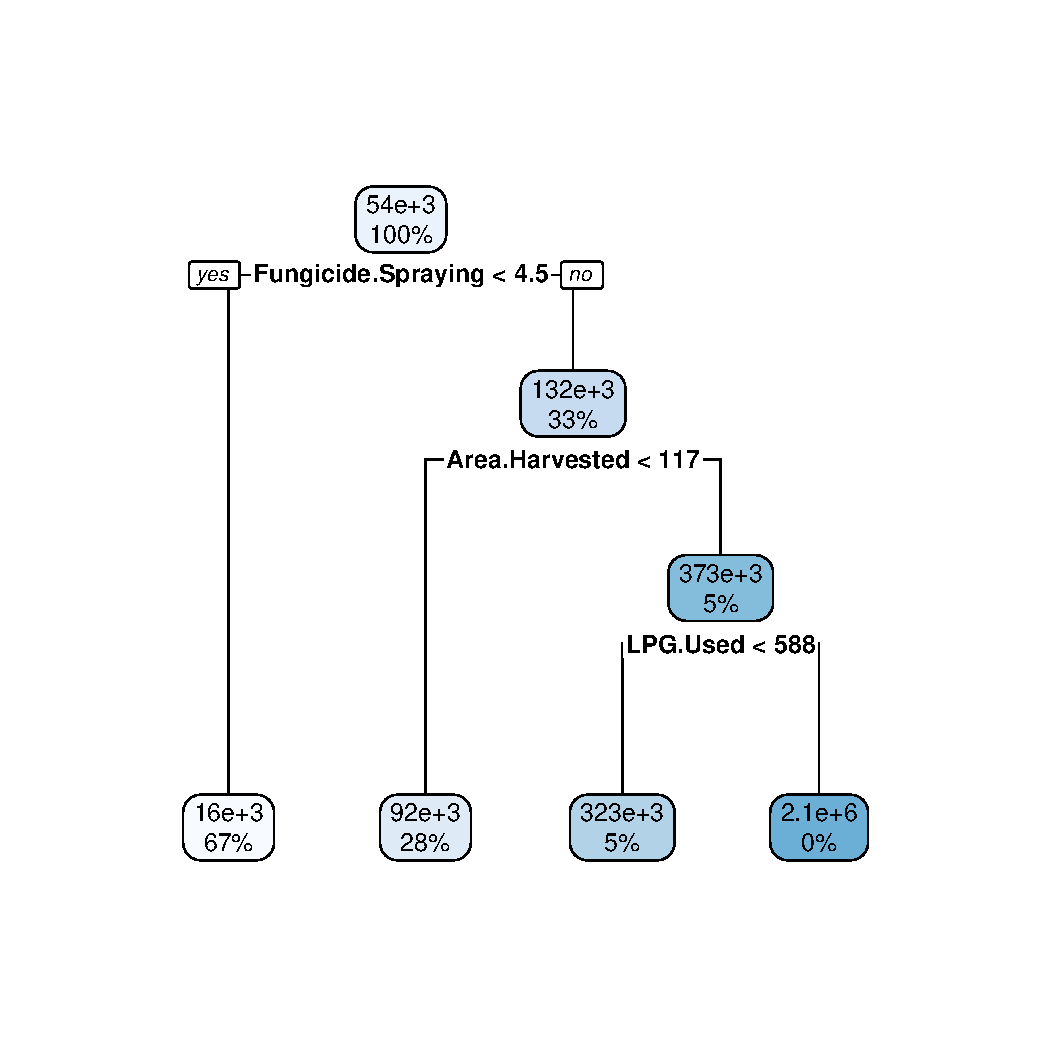
\includegraphics{revenue.pdf}}
%   \caption{Decision tree predicting revenue. Each node indicates the class predicted, and the proportion of elements agreeing with nodes partitioning, with the left direction indicating a yes to the nodes rule.}\label{fig:revenue_tree}
%  \end{figure}
 
The predictive performance of the XGBoost model for revenue performed similarly to operating cost, for achieving an $R^2$ of 0.77 (with a standard deviation of 0.15). 
\par
The most important predictors of revenue were fuel use (petrol 307 and diesel 144), yield (285), size (216) and water use (199). The values attached to each variable indicate the relative importance of the variable (number of times selected in the tree ensemble, see Section \ref{fig:revenue_sankey}). Overall regions contributed to 234 nodes in the ensemble making them collectively the third most important variable. The chord diagram (see Figure \ref{fig:revenue_sankey}) illustrates that vineyard area is also of high relative importance to other variables, especially slashing. The overall importance of Area to other variables is evident by its larger circumference within the chord diagram.
% The strong relationship of vineyard area to revenue and its predictors  but also has a high relative importance to the other predictors, The relation to area is likely to primarily be the effect of economies of scale, shown through its strong relations to other variables in figure \ref{fig:revenue_sankey}. Area harvested is likely also an indicator of other variables such as slashing passes its strongest connection presented.

\begin{figure}[htb]
  \label{fig:revenue_sankey}
  \resizebox{\textwidth}{!}{
  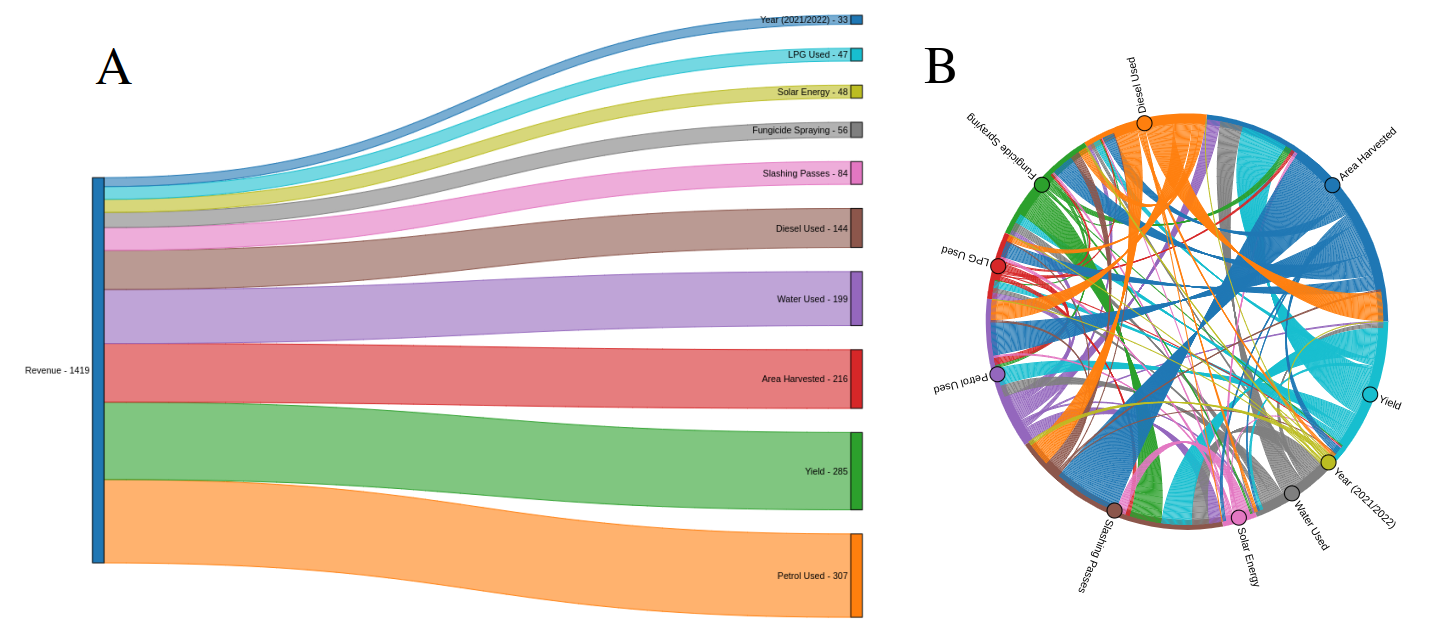
\includegraphics{revenue.png}}
  \caption{The left-hand side depicts the 10 most important variables in predicting revenue using XGBoost as a measure of node occurrence, using a Sankey diagram. The right-hand side depicts the interrelated importance of the ten predictor variables using a chord diagram.}
 \end{figure}

\subsection{Operating Costs}

% \begin{figure} 
%   \resizebox{\textwidth}{!}{
%   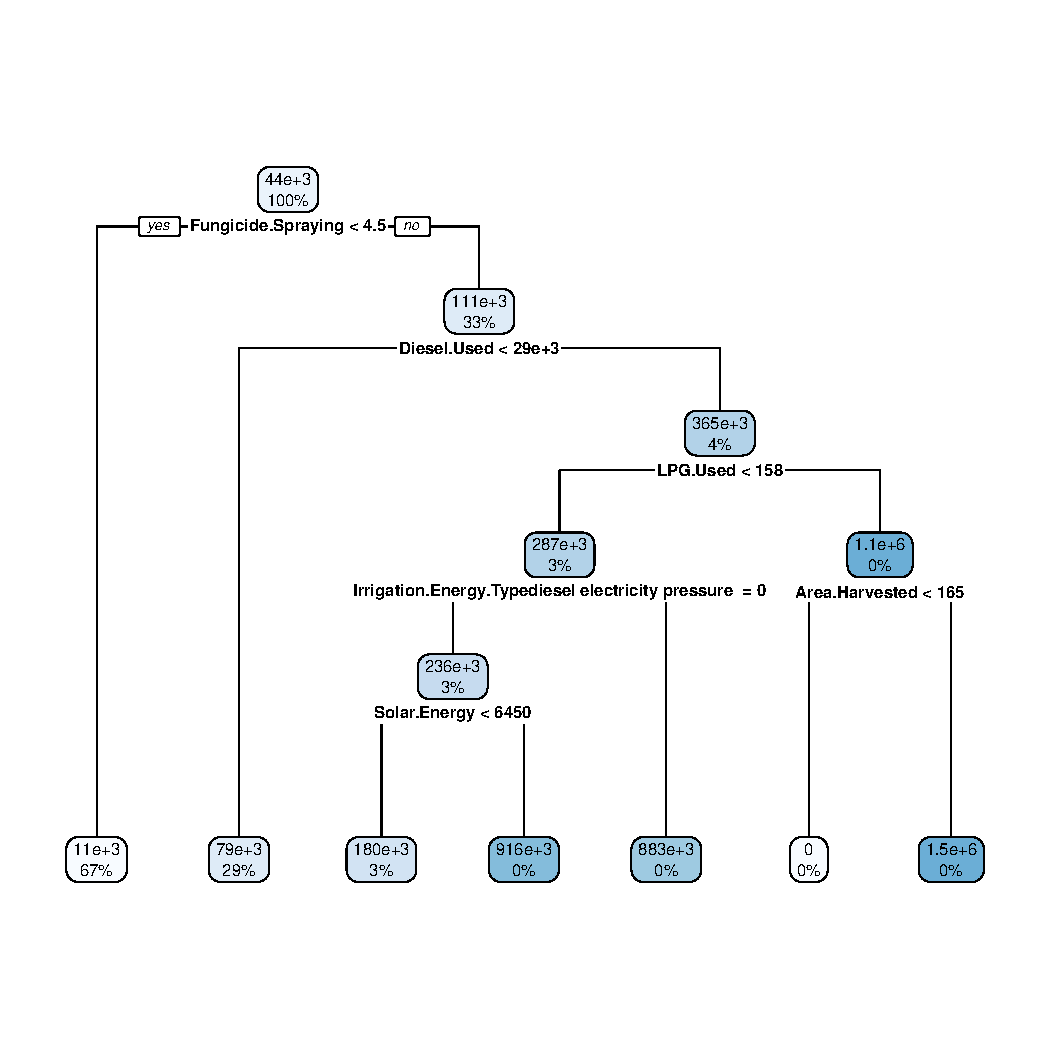
\includegraphics{operating_costs.pdf}}
%   \caption{A surrogate model decision tree predicting operating costs. Each node indicates the class predicted, and the proportion of elements agreeing with nodes partitioning, with the left direction indicating a yes to the nodes rule.}\label{fig:operating_tree}
%  \end{figure}

Compared to revenue, the predictive performance of XGBoost model for operating cost was slightly better, with an $R^2$ of 0.80 (with a standard deviation of 0.10). Similar to revenue, the most iomportant predictors of operating cost were fuel, water, area and yield (see figure \ref{fig:operating_costs_sankey}). A surprising difference was the change in relative importance of activities involving tractor passes where the use of fungicide was more important for operational costs, compared to revenue, where slashing was more important (see Figure \ref{fig:region_sankey}). The variables that feed into these decisions are also very different with diesel having the highest relative importance to slashing, and area having the greatest relative importance to the need for fungicide.
\par
Again, Region played a determining factor overall, contributing to 334 nodes within the ensemble making it the most important variable when considering all regions together. It was surprising that electricity, slashing and spraying passes were not more prominent in operating costs due to the intrinsic nature as an agricultural expense.
\par
% . Again the surrogate model did not perform well achieving an $R^2$ of 0.0931 (with a standard deviation of 0.0197) but showed similarly to revenue an importance placed on fungicide spraying and size (see figure \ref{fig:operating_tree}).
\begin{figure}[htb]
  \resizebox{\textwidth}{!}{
  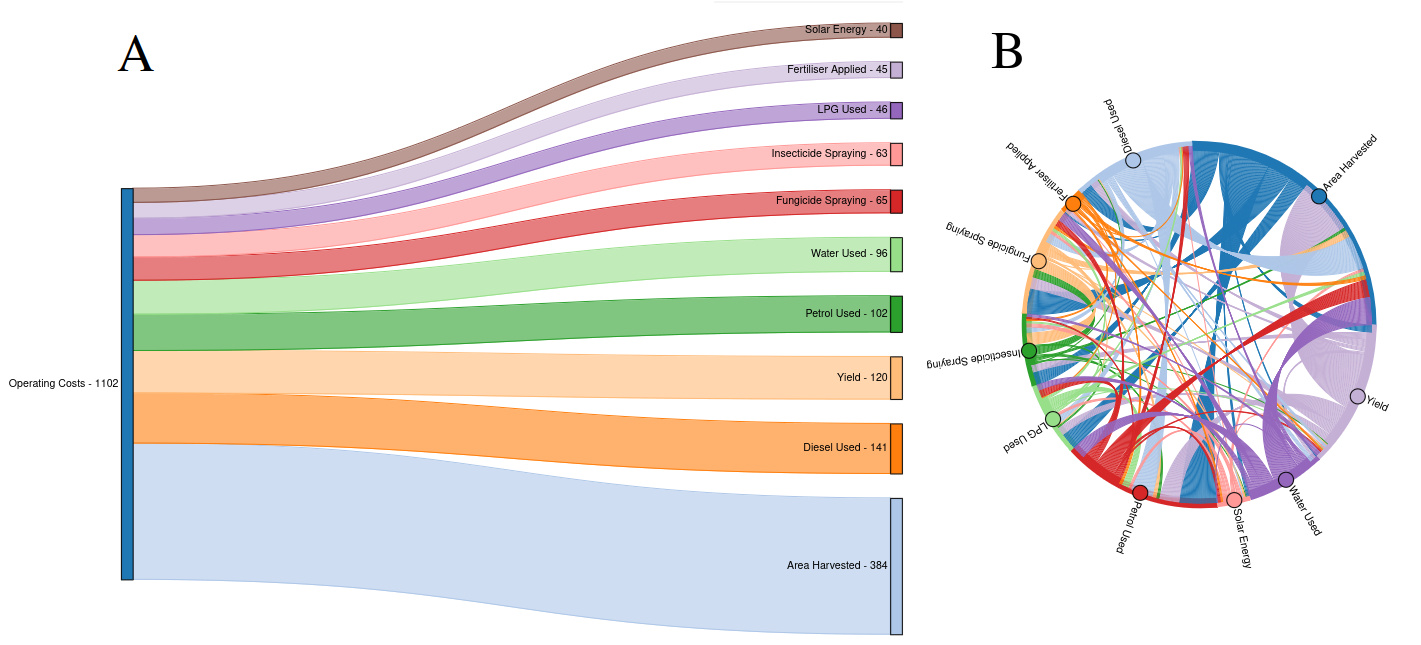
\includegraphics{operating_costs.png}}
  \caption{The left-hand side, A,  depicts the 10 most relative  important variables in predicting Operating Costs using XGBoost as a measure of node occurrence, using a Sankey diagram. The number at the end of each band in the diagram is that variable's importance. The right-hand side, B, depicts the importance of the 10 variables in Sankey diagram relative to one another.}\label{fig:operating_costs_sankey}
 \end{figure}


\subsection{Region}

% \begin{figure}
%   \resizebox{\textwidth}{!}{
%   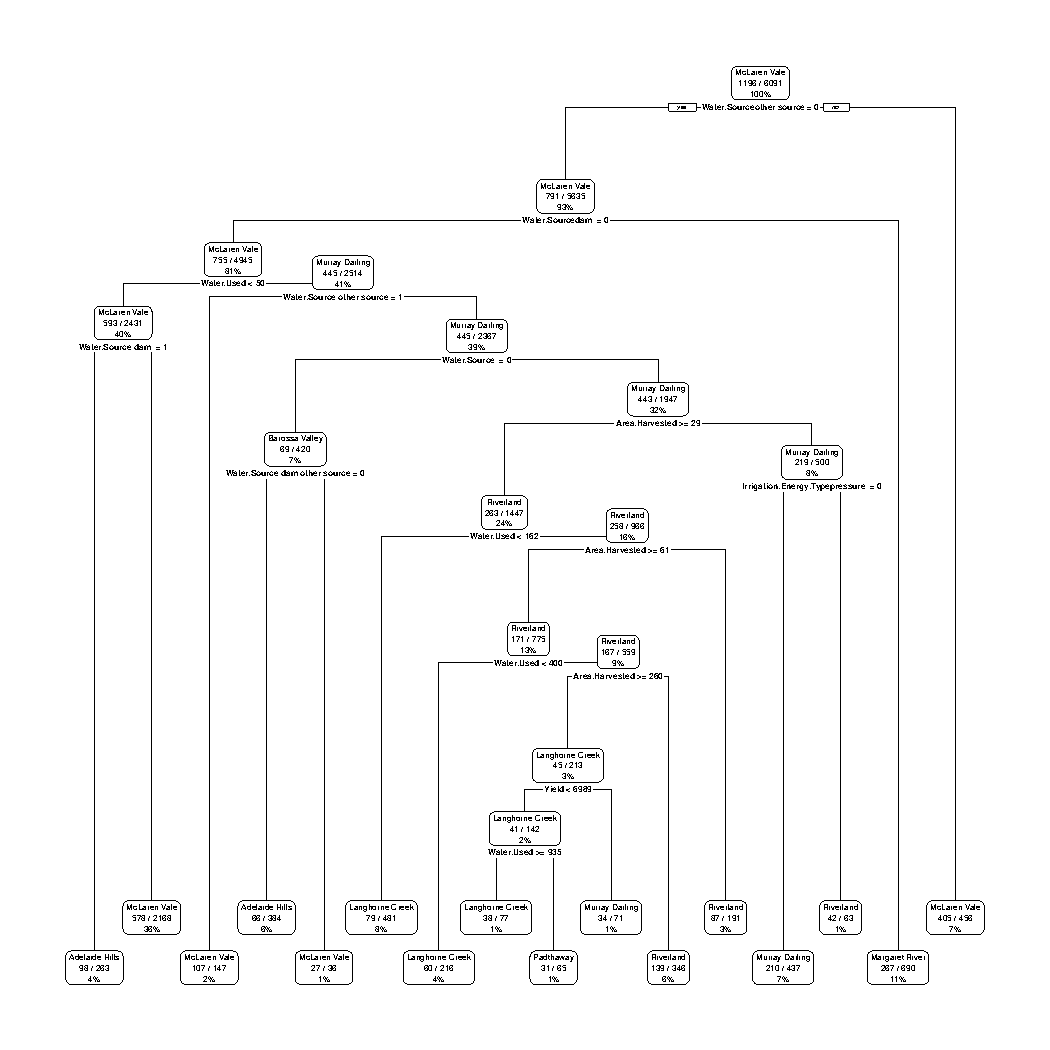
\includegraphics{region.pdf}}
%   \caption{Decision tree predicting Region. Each node indicates the class predicted, and the proportion of elements agreeing with nodes partitioning, with the left direction indicating a yes to the nodes rule.}\label{fig:region_tree}
%  \end{figure}
 


Region was a highly informative variable based on measures of importance for both operating cost and revenue. As noted above, Region was the third most important variable for determining revenue. The Barossa Valley region and Tasmania were the two most important regions in relation to revenue; these two regions are considered to be some of the highest revenue per hectare regions in Australia \citep{wineaustraliaNationalVintageReport2022}. These two regions are also relative opposites in winegrowing climates with the Barossa having a warm and dry climate focussing on Shiraz grapes and Tasmania having a cool wet climate that favours Pinot/Chardonnay \citep{wineaustraliaNationalVintageReport2022}.
\par
As also noted above, Region was also a key determinant of operating costs. Tasmania had the highest relative importance, followed by the Adelaide Hills. In contrast, the regions of the highest relative importance were warmer and drier, such as the Barossa. The higher relative importance of fungicide spraying is the likely due to fungal pressure being greater in cooler wetter regions variables than in drier regions.
\par
The XGBoost ensemble for Region achieved an accuracy of 56.82\% (and 50.58\% validation accuracy). The difference in accuracy compared to the other models is in part due to the large number of classes (58 regions). The ensemble had an emphasis on area, water, fuel and yield as determining factors (see Figure (\ref{fig:region_sankey}).
% Although water and diesel were two of the three most frequently occurring variables in predicting region, they were not as connected to the other predictor variables as Yield and area harvested were.
\par
A number of regions had lower reporting rates, resulting in much poorer classification performance. The regions with the most samples performed the best likely due to the disparity in sample sizes. Bordering regions were routinely grouped together and misclassified as the same region. When scrutinising each class explicitly, the two areas that effected the most from this were the Limestone Coast (cool coastal areas in South Australia) and the warmer inland regions along the Murray Darling.

\begin{figure}[htb]
  \resizebox{\textwidth}{!}{
  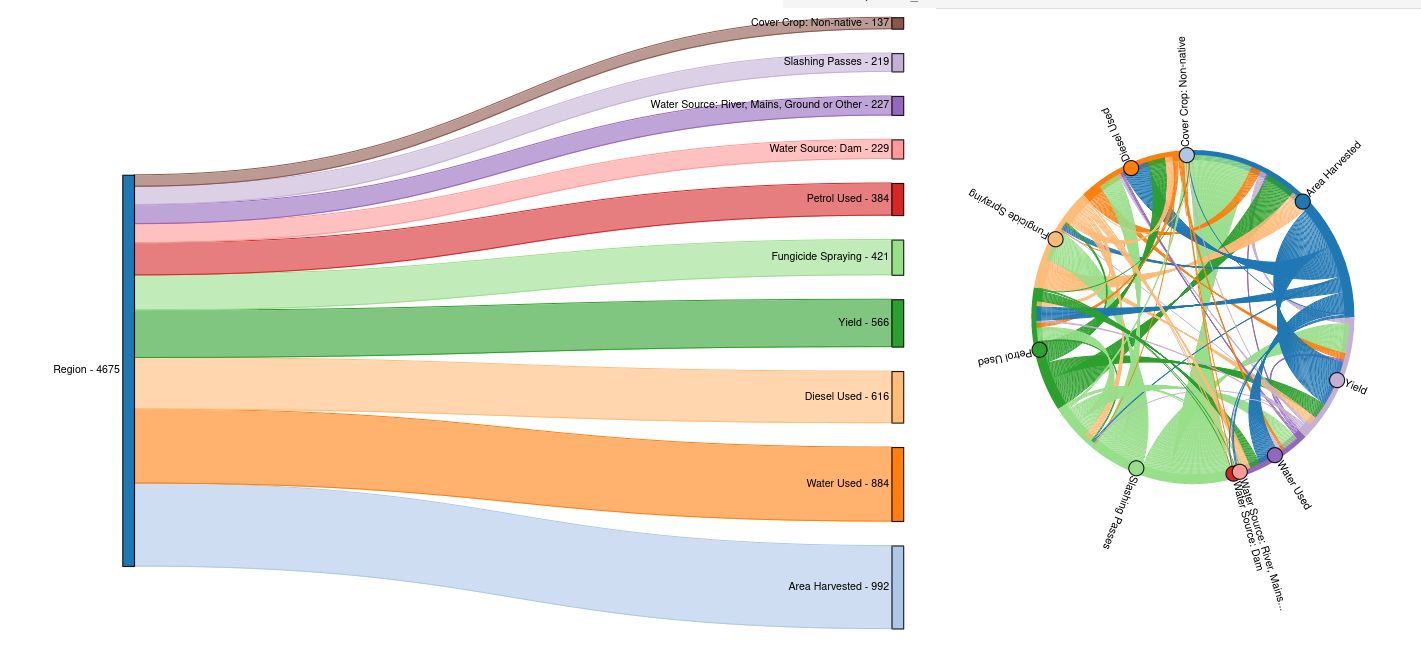
\includegraphics{region.png}}
  \caption{The left-hand side, A,  depicts the 10 most relative important variables in predicting Region using XGBoost as a measure of node occurrence, using a Sankey diagram. The number at the end of each band in the diagram is that variable's importance. The right-hand side, B, depicts the importance of the 10 variables in Sankey diagram relative to one another.}\label{fig:region_sankey}
 \end{figure}
\section{Discussion}

This study explored the relationships between vineyard resource use, operations and geographical properties to revenue and operating costs. The analysis was based on a large national study of 6049 samples collected over ten years. Three main findings were identified. First, the most important predictors of revenue and operating costs were fuel, yield and area. Secondly, area and fuel were highly interrelated to other variables (see Figure \ref{fig:operating_costs_sankey} and Figure \ref{fig:revenue_sankey}A). Finally, the relative importance of predictor variables for Region, differed from Revenue and Operating costs, with Water Use being more prominent than Yield. Region was also more prominent than illustrated in the Sankey diagrams due to the relative importance for operating cost and revenue being calculated for individual regions and not all regions together. In its entirety Region was the third most important predictor of revenue and the most important predictor for operating costs, relative to the other variables consideration in the analyses.
\par
Several physical parameters such as climate, geography and soil are predetermined by a vineyard's location, making it a widely considered key determinant of grape yield and quality \citep{abbalDecisionSupportSystem2016,agostaRegionalClimateVariability2012,fragaMultivariateClusteringViticultural2017}.
The association between yield and region is demonstrated by yield apparing as the fourth most important variable when determining region (see Figure \ref{fig:region_sankey}).
% The association with area and region is likely a connection to the change in land costs, with inland Australian areas (particularly of lower rainfall) being substantially cheaper to buy than coastal regions, allowing larger areas to be purchased \citep{willchancellorMeasuringAustralianBroadacre2019} % TODO: This section is commented out due to Mardi's take:
%  Maybe but not sure this assumption holds. It may be an artefact of the members being corporate in larger holdings. The larger percentage of blocks in the riverland are small.
\par
Warmer regions are known to be beneficial in hastening the ripening process of winegrapes \citep{webbObservedTrendsWinegrape2011}. Warmer regions are also associated with lower quality grapes, caused largely due to this hastened ripening \citep{botting1996canopy}. It is likely that the combination of larger vineyards with higher water use is a determining factor in classifying regions which favour larger production of grapes; reflected through region using water use so prominently in the XGBoost ensemble. The link to water resources in defining regions is also an important consideration, as vineyards can leverage higher irrigation rates if water resources are available. A further consideration in the link between revenue and region is that grape prices are set at a regional level by buyers \citep{wineaustraliaNationalVintageReport2022}. It is also important to consider that some regions carry particular fame regarding the quality of their produce such as Tasmania, the Hunter Valley and Barossa Valley \citep{hallidayAustralianWineEncyclopedia2009}. This classification can be contrasted with other warmer regions of higher rainfall that use the warmer climate to concentrate their grapes, increasing the flavour profile \citep{goodwinijeriepRegulatedDeficitIrrigation1992,mgmccarthyEffectCropLoad1986}.
\par
In part, yield is sometimes restricted simply through access to water resources. Regions are likely to have varying access to different water sources, such as those along the River Murray being able to utilise river water for crops, unlike most coastal regions which may be drawing from surface or underground water sources. Similarly, the connection between region and fuel use is likely an indicator of the level of infrastructure within the region because vineyards in regions without pressurised water will need to use more fuel or electricity to pressurise their irrigation systems.
\par
Operational costs showed similar importance across fuel, water and tractor use. The dominating factor of area likely played a large part in determining how costly a tractor pass would be, or in defining the ratio of water applied to the amount of vines. The relative importance was high for area but much lower in general across the other variables, which could indicate the need to be specific when attempting to determine the cause of a operational cost. Although these analyses attempted to capture the complexity between how variables interacted when determining operational costs (see Figure \ref{fig:operating_costs_sankey}), in reality these relationships are likely even more complicated. An example of how interrelated operational costs can be, is 
the optimisation of tractor passes to achieve multiple goals in a pass, being shown to reduce energy use in vineyards, decreasing running costs, as well as reducing soil compaction \citep{capelloEffectsTractorPasses2019}. 
\par
When determining revenue, similar variables were used to operational cost; with region also being of high variable importance relative to other variables (when considering all regions together in importance). It is difficult to extrapolate the specific influence of location on a vineyard's outcomes due to the broad and varying definition of a region. Utilising the Geographical Indicator regions defined by Wine Australia \citep{wineaustraliaWineAustraliaOpenData2021} is a limitation in one way, as it is too broad to fully capture a vineyards location and how that influences variables at a more granular level. However, as buyers set prices at regional levels, it is still important to consider this factor. 
\par
Decisions made on the ground have far-reaching effects and are difficult to completely capture. A larger number of tractor passes used as a preventative measure for occurrences such as disease may incur higher operational costs but could be critical in preventing long term losses. Although the models demonstrated a good predictive fit (via large $R^2$ values), the ability to predict operational costs is limited by the variables incorporated in the analysis. Other factors such as erosion and soil health are also influenced by tractor use and would contribute to these operational costs but are difficult to measure and were not available as part of the data \citep{capelloEffectsTractorPasses2019,capelloPermanentCoverSoil2020}. Reductions in fuel, water and tractor use are obvious methods to reduce operational costs but not necessarily achievable decisions. Without fully capturing more granular activities for example the specific reasons for fuel use, it is difficult to determine what decisions specifically influence the operational costs.
%  Electricity in particular is used predominantly for irrigation. 
% Size is also a further consideration where slashing and spraying are measured in discrete tractor passes and show a surprising connection to the overall size of a vineyard, despite not being scaled to any measure of size. This would mean that, although measured as the same increment, a slashing or spraying pass in a larger vineyard would consume more fuel and wages than in a smaller vineyard.
\par
The reasoning for any particular decision can be widely varying. 
% Where, a cover crop may be employed to help increase soil water retention, reduce erosion, increase biodiversity and reduce weeds \citep{capelloEffectsTractorPasses2019,capelloPermanentCoverSoil2020,delpuechAdaptingCoverCrop2018}. However, cover crops can introduce competition with grapevines and may reduce yield depending upon the plants used and the density of the cover crop \citep{goslingLongtermChangesSoil2005,monteiroInfluenceCoverCrop2007}. 
% A more granular definition of region may help to better discern the differences in practices, and the reason for employing them. 
More sophisticated models, specifically those that utilise expert opinion, may also help to capture and address the decision-making process. An example is the optimisation of fungicide sprays using Bayesian models that forecast disease risk \citep{luDiseaseRiskForecasting2020}. 
\par
% It is reasonable that regions, being subjected to different rainfalls and temperatures, would require different amounts of water, and would have access to different water sources. The relation of area harvested and fuel (particularly petrol) is prominent with other predictors. Due to the wide variety of uses of petrol and diesel. It is likely that fuel use is representative of other activities within the vineyard, such as pruning and harvesting. Predictors such as yield and area being highly interconnected to fuel are likely reflective of fuel required to  as they likely operate as proxy variables to other factors, possibly other present variables.

% In particular There is the potential that the types of herbicides used also have a long term effect on crops, reducing the presence of microorganisms and soil health, making the area more prone to disease in the long run, becoming dependent on these sprays (Coll et al., 2011; Gosling and Shepherd, 2005).

% The classification tree shows a likely change in avaialble infrastructure across the years, with mroe current years being associated with pressurised water and more slashing and herbicide passes.

% The availability of solar panels for electrical irrigation and electrical irrigation in general

% Electricity is predominantly used for pumping and irrigation in vineyards \citep{longbottomRoleVineyardPractices2015}

% Fungicides are likely associated with higher preventive sprays when disease breaks out.

% Slashing passes are likely weed outbreaks or yearly cycles?

% %% Climate change

% %% Pests Insects and weeds
% %% Disease

% %% Electricity use and reasons for (connect to year)
% %% Fuel use and what it is used for

% Operational costs saw the only occurrence of renewable resources being included in the ten most important variables for its XGBoost ensemble. 

% %% Address yield and how predictable it is
% %% different sales markets and performance?
% %% Reasons for profit?

% The winegrowing industry holds significant importance for Australia and its economy. There exists many challenges that the industry has to contend against, 
% with disease from sources such as Mildew and Botrytis being a considerable one (Cole, 2010; Magarey et al., 1994).

Separately, revenue and operating cost did have a greater predictability than their counterpart profit (see Appendix). The disparity in accuracy between profit and other economic outcomes is reflective of the complexity in trying to address challenges such as climate change, disease and changing market demands \citep{wineaustraliaNationalVintageReport2020,wineaustraliaNationalVintageReport2021,wineaustraliaNationalVintageReport2022}. The difference between turning a profit or loss is dependent on predictable factors unforecasted factors, farming practice and farmers' decisions. The difference between vineyards that make profit and those that do not could be a multitude of factors including differences in farming practices not captured within this study.
\iffalse
%%%%%%%%%%%%%%%%%%%%%%%%%%%%%%%%%%%%%%%%%%%%%%%%%%%%%%%%%%%%%%%%%
%  Prior studies have shown that decisions can also have long-lasting positive effects at the cost of short term negatives. In particular the use of cover crops and remedial soil techniques offer such as trade. 

% with well established a cover crops requiring greater water resources to maintain but offering more protection in return (Capello et al., 2019; Delpuech and Metay, 2018; Gosling and Shepherd, 2005; Monteiro and Lopes, 2007). 

% Prior studies have placed an emphasis on optimisations of fungicide sprays through the development of Bayesian models to forecast disease risk (Lu et al., 2020). This analysis investigates at the synergy between spray strategies as a proxy of fuel use to different types of water sources and sustainable strategies with an emphasis on the use of cover crops; allowing for the modelling of interactions between the use of multiple strategies. With the need to balance yield, quality, and combat adversities such as disease; the creation of tools to inform decisions and assist growers with warnings of disease risks is becoming crucial in ensuring sustainable and profitable wine production (Abbal et al., 2016).

% Soil is an important and ongoing consideration for vineyards and interacts with every other practice in various ways at different time scales. For example, cover crops have been shown to be detrimental for soil health in the short term, giving an initial reduction in soil potassium and phosphorus concentrations and no change in nitrogen levels (Gosling and Shepherd, 2005). Conversely, in longer time frames the presence of a cover crop can induce an increase in microorganisms, which can excrete phosphates and potassium, regenerating the soils chemical balance and helping to introduce further organic nitrogen (Coll et al., 2011). The studies that showed this were based in two different countries of similar climate but could have been subject to other underlying conditions not measured. 

% When implementing practices such as cover crops the extent of the practice, the compounding effects and potential alternatives need to also be considered. Alternative options are always available such the use of mulch and wood chips to increase soil health and water retention in place of more involved processes such as crop rotation (Rössert et al., 2022). Crop rotation offers greater benefits than other soil management plans (Brock et al., 2011), however this is often not a viable option for many vineyards although is common practice in some places (Russo et al., 2021). The need to look at the holistic outcomes and interactions of these practices is paramount, however with the existence of many different practices, the outcomes due to interactions are not always known; one such consideration is the use of fungicide and its potential to build up copper, causing a reduction of microorganisms in the soil. Linking copper build up to any particular cause is a difficult endeavour due to the need for multiple reliable soil samples which are equally effected by the same conditions, within soil (Wightwick et al., 2010). 

% Reasons for operational costs (connect to disease and pests)

% There are several environmental concerns that affect viticulture, including loss of soil quality, lack of rain, hail, disease, fire, and frost; with climate change exacerbating these issues. In 2020, 40,000 tonnes of grapes were lost across 18 different wine regions due to bush fires and smoke taint; the predicted incidence of wildfires is expected to increase (Canadell et al., 2021). In comparison to countrywide pressures such as drought, this damage made up only 3\% of the total amount of grapes for that year; although acknowledged as a considerable loss on an individual basis, it was deemed to be only a minor national concern by Wine Australia when compared to other environmental pressures such as drought (Wine Australia, 2020). 

% In rainfed areas due to the lack of irrigation possibilities The result would be a shortening of the ripening period, with harvest occurring during the period with high temperatures, which could have a negative impact on wine quality (Salazar Parra et al. 2010; Duchne and Schneider 2005; Jones and Davis 2000) and yield (Mira de Ordua 2010; Iglesias et al. 2010).

% Climate change in the future might move the north and south latitude boundaries of areas suitable for good quality wines (Schultz and Jones 2010), and could even lead to improvements in fruit production and quality in some areas (Olesen and Bindi 2002). However, other areas may be negatively affected by high temperatures and water stress due to a reduction in the amount of water available. 


% %% Grape quality

% The difference between grape quality is most notable between warm inland regions and coastal regions such as the Riverland and Coonawarra, respectively. Grape quality is only described by a singular variable within this study, however in reality it is driven by market demand and subject to complex forces such as international market pressure, fire, pests and disease (Wine Australia, 2022, 2021, 2020, 2019; Winemakers’ Federation of Australia, 2018, 2017, 2016, 2015, 2014, 2013, 2012).

% The decision trees were able to offer some insights into the factors that influence grape quality and regional contrasts that contribute to different qualities. The most prominent being what readily available resources of each region were, particular the types of water available. Heavy water consumption is often linked to the mass production of grapes, where lower quality grapes are targeted in a quantity over quality strategy. These types of business decisions are unfortunately obfuscated by lack of in-depth data regarding vineyard business plans. Notably the literature shows that there are many complex decisions to be made on the ground depending on many compounding factors that influence both quality and yield ((Abad et al., 2021; Cortez et al., 2009; Hall et al., 2011; I. Goodwin, et al., 2009; Kasimati et al., 2022; Oliver et al., 2013; Srivastava and Sadistap, 2018)). There are also further differences when comparing winegrowers to other agricultural industries as they are vertically integrated within the wine industry, tying them to secondary and tertiary industries, such as wine production, packaging, transport and sales. This results in unique issues, where on-the-ground choices are influenced by other wine industry’s decisions, such as the use of sustainable practices in vineyards to sell in overseas markets; notably these interactions are further complicated by some winegrowers being totally integrated into wine companies, while others are not (Knight et al., 2019). It is incredibly difficult to attribute external business decisions to produced grape quality but it is important to acknowledge that some growers are contracted to produce grapes of a particular grade; it is difficult to know whether another consumer may have graded the grape quality differently paying more or less for the same grapes given the opportunity to purchase them. It is difficult to untangle the contributing factors to the success of winegrowers and the quality of grapes produced without further specifics of choices made through out a season (Leilei He et al., 2022).

% %% connection to watrer resource availability
% What are the water resources in the hunter valley and tasmania?

% economic pressures

% Historically strong demands for Australian wine have helped to create a thriving industry, however recently sharp reductions in exports to mainland China due to significant deposit tariffs have caused a decline of 19% in Australian export value during the 2021-2022 financial year (see Figure 1) (Wine Australia, 2022). The pressure brought on by the drop in export value has been exacerbated by loss of tourism and labour due to the COVID-19 pandemic, global freight crisis, war in Europe and rising inflation (Wine Australia, 2021a, 2020). These pressures within the wine industry have trickled down to vineyards, where winemakers retain unwanted wine, creating an oversupply of grapes. Currently the proposed strategy to soften pressures proposed by Wine Australia includes initiatives focused on market diversification, and sustainability to build resilience in the coming years. 

% Figure 1: The exports of Australian wine over time in Australian Dollars Free On Board, comparing exports between China and the rest of the world. This graphic is taken from the Wine Australia Annual Report of 2020-21(Wine Australia, 2022).

%%%%%%%%%%%%%%%

% %Two regions, the Riverland and Coonawarra, were the most accurate classes being 92.74% and 96.97% respectively. 

% These regions differ greatly in practice and geophysical properties, with the Riverland being a dry warm inland region and Coonawarra being a cooler, wet coastal region. However, they are both similar in operational scales, with vineyards being relatively large compared with other regions. The differences in resources and practices between these regions are also significant, such as the Riverland utilising the river Murray as a water source. 

% The difference between grape quality is most notable between warm inland regions and coastal regions such as the Riverland and Coonawarra, respectively. Grape quality is only described by a singular variable within this study, however in reality it is driven by market demand and subject to complex forces such as international market pressure, fire, pests and disease \citep{wineaustraliaNationalVintageReport2019,wineaustraliaNationalVintageReport2020,wineaustraliaNationalVintageReport2021,wineaustraliaNationalVintageReport2022,winemakersfederationofaustraliaNationalVintageReport2015,winemakersfederationofaustraliaNationalVintageReport2016,winemakersfederationofaustraliaNationalVintageReport2017,winemakersfederationofaustraliaNationalVintageReport2018} % The original citation included years prior to this dataset just be casreful with this. It is a bit unclear what you are really trying to cite and its relevance. I think it important to chop this up.

% The decision trees were able to offer some insights into the factors that influence grape quality and regional contrasts that contribute to different qualities. The most prominent being what readily available resources of each region were, particular the types of water available. 
% A citation or reference to a study looking at the disparity in wine regions and their resources - or use the data more to describe these regional differences. Is water availability apparent? Do some regions have access to more sohpisticated water sources such as pressurised water etc.

%  Heavy water consumption is often linked to the mass production of grapes, 
 
 % Really? proce it? Where in the results is this really found?? This sounds like a link to your previous paper but you cannot really show this and you do not really produce evidence to support this claim.

%  where lower quality grapes are targeted in a quantity over quality strategy. These types of business decisions are unfortunately obfuscated by lack of in-depth data regarding vineyard business plans. 

 % This point is incredibly important but it, itself, is obfuscated by you odd claims that are not supported by facts. Better to talk about how this could improve and the weaknesses than to start spouting unsupported claims.

%  Notably the literature shows that there are many complex decisions to be made on the ground depending on many compounding factors that influence both quality and yield \citep{abadCoverCropsViticulture2021,cortezUsingDataMining2009,hallWithinseasonTemporalVariation2011,i.goodwinManagingSoilWater2009,kasimatiPredictingGrapeSugar2022,oliverReviewSoilPhysical2013,srivastavaNondestructiveSensingMethods2018}
 % Woah woah woah
%
 % what are these decisions??? Slow down speed gonzales!! This is really interseteing and important. Discuss it, its the discussion! God damn I want to know and I wrote this!.
 %
%
% This is not all one paragraph surely! There are so many ideas here that should be discussed!
%
% This leads heavily into the next paper and shows that natural progression. Especially in the sense of: if regions have so much influences, what determines ones use of water, fertiliser, etc. And, what determines the success financially, in quality or quantity? How are thes evariables interacting! The next paper is less about predicting and much more about what interacts with what? Where as this paper is about how things change over landscapes and what localised events helpe to determine decisions and their outcomes.
%
%  . There are also further differences when comparing winegrowers to other agricultural industries as they are vertically integrated within the wine industry, tying them to secondary and tertiary industries, such as wine production, packaging, transport and sales. This results in unique issues, where on-the-ground choices are influenced by other wine industry's decisions, such as the use of sustainable practices in vineyards to sell in overseas markets; notably these interactions are further complicated by some winegrowers being totally integrated into wine companies, while others are not (Knight et al., 2019). 

% This is an interesting point. However it would be better to include other industries, such as the ones you touch on in your previous chapter. If industries such as Sake are similar - how do their decisions effect the outcomes of rice quality and Sake? A point of comparison and difference would be great here! 

%  It is incredibly difficult to attribute external business decisions to produced grape quality but it is important to acknowledge that some growers are contracted to produce grapes of a particular grade; it is difficult to know whether another consumer may have graded the grape quality differently paying more or less for the same grapes given the opportunity to purchase them.

% What are these business decisions? Can you give some examples?

%  It is difficult to untangle the contributing factors to the success of winegrowers and the quality of grapes produced without further specifics of choices made through out a season \citep{leileiheFruitYieldPrediction2022}.

% It is difficult yes, but please at least try! Highlight some of these affects, some of these different contributing factors! What did we really learn by doing this? What can someone take away from this and say thank you for? (like Josh said)


% \subsection{Model 1 GI Regions}

% The first Model was used to classify GI regions
 % Interestingly the firs I am hearing of this - each model needs to be more well summarised. A table would be good.

% and resulted in an accuracy of 36.48\% across 52 classes. The most prominent features used to classify regions were the types of water resources available (see Figure 1). Two regions, the Riverland and Coonawarra, were the most accurate classes being 92.74\% and 96.97\% respectively.

% it might be worth only talking about the regions that were well classifified - and then talk about their determining traits.

% These regions differ greatly in practice and geophysical properties, with the Riverland being a dry warm inland region and Coonawarra being a cooler, wet coastal region. However, they are both similar in operational scales, with vineyards being relatively large compared with other regions.

%Summary statistics regarding these two regions would be a better point of comparison, for example:
%
% How much in size do these operational scales differ?
% How much yield do they differ by?
% What are the differences in rainfall etc
% What makes them unique, different and similar?
%

% The differences in resources and practices between these regions are also significant, such as the Riverland utilising the river Murray as a water source.
% What are the specific differences? This is a really critical part of this paper

% Many of the regions had significantly lower reporting rates, resulting much poorer classification performance.
 % This is almost its own paragraph. Why was this case? is it important? what are the similarities and differences of regions that were poorly classified?

%  The regions with the most samples performed the best (see Table 1). Notably bordering regions were routinely grouped together and misclassified as the same region, for example the two closest regions to Coonawarra, Padthaway and Wrattonbulley, were misclassified as Coonawarra even though they had 147 and 137 samples respectively. The same case was found for the Murray Darling, with 143 samples, it was misclassified as the Riverland.
 % This speaks highly to why regions were poorly classified.

% These misclassifications are likely due to the incredibly similar regional properties and close proximity these regions have with one another. Other misclassifications were most likely due to lower reporting rates with many regions being under represented.

% \begin{table}[]
%   \caption{Classification accuracy of the most prominent GI Regions.}
%   \label{tab:accuracy}
%   \resizebox{\textwidth}{!}{
%     \begin{tabular}{@{}llll@{}}
%       \toprule
%       \textbf{} & \textbf{Accuracy} & \textbf{Predicted} & \textbf{Actual} \\ \midrule
%       \textbf{Adelaide Hills} & 30.45\% & 95 & 312 \\
%       \textbf{Barossa Valley} & 51.00\% & 205 & 402 \\
%       \textbf{Coonawarra} & 96.97\% & 192 & 198 \\
%       \textbf{Langhorne Creek} & 22.84\% & 53 & 232 \\
%       \textbf{Margaret River} & 78.82\% & 201 & 255 \\
%       \textbf{McLaren Vale} & 52.89\% & 128 & 242 \\
%       \textbf{Riverland} & 92.74\% & 345 &
%     \end{tabular}
%   }
% \end{table}

% \subsection{Climate}
% Classifying the SWA climatic categorisation of the given regions had better performance than the GI Regions, with ~41.66\% being classified correctly. These categories were divided into 12 climatic classifications with 3 and 4 separate subsets for rainfall and temperature respectively. The decision tree behaved similarly and over classified climates with higher response rates. The results posed an interesting similarity with grape quality classifier, being influenced predominantly by water and area. The use of fungicide to separate regions that were 'Very dry' and 'Damp' can be considered as indicative of the different practices required due to climatic pressure; fungicides being more prominent in cooler regions with greater rainfall due to the higher risk of disease pressure \citep{reynoldsManagingWineQuality2010}. % interesting although not really appropriate for the results section.
%  This could also potentially explain the use of contractor tractor use to discern differences in grape quality, where the lack of contractor use to prevent disease could have led to lowered quality of grapes.

% You really need to show every decision tree.

% \subsubsection{Rainfall}
% The rainfall decision tree showed a greater use of fungicides sprays to discern between damp and very Dry as shown in Figure 4; with the accuracy improving to 62\% but was unable to effectively discern between dry and very dry regions (see Table 3).

% was again used to differentiate between warm and cool regions, likely being due to disease pressure. The temperature classification tree

% \subsection{Model 3 Grape Quality}
% The classification of grape quality through its grade % It might even be worth considering this as pseudo grade - or better define it in some of the australian wine journals rose suggested.
% had an accuracy of 55.72\% across 5 separate grades. There was a notable issue with the classification of B grade grapes when compared to A and C (see Table 2). % This is actually really interesting.
%  The classification tree itself shows similarities to that of classifying regions in Model 1, with the type of water resource used being a prominent determiner. Although not surprising the number of contractor tractor passes is new deciding factor due disease and pests reducing the potential quality of a crop. The prevalence of contractor use is greater in regions such as the Barossa Valley and the McLaren Vale, this could be due to the difference in operational scales, with larger sites being more likely to have ownership of their own equipment for weeding and spraying due to the cost benefit.

\fi

\section{Conclusion}

This study has provided valuable insights into the multifaceted dynamics governing operational costs and revenue in vineyards. The impact of different regions highlighted the complex interrelatedness of variables within a vineyard. We relate how factors such as water and fuel intersect to impact operational costs and how different seasonal events affect these operations; as well as the significance of context-specific decision-making. While this investigation utilised a broad regional classification, the potential benefits of adopting a more nuanced approach and incorporating expert knowledge have been highlighted. Further work could pursue causal models and the creation of decision support systems. It is difficult to untangle the predictive and correlative nature of a variable compared to the causal reasons. By delving deeper into the complex interplay of variables, further advancements can be made in optimising vineyard management strategies for lowering operational costs, increasing revenue and enhancing sustainability.

% The intricate relationships between water resources, and management practices have been examined through advanced techniques like XGBoost ensembles, shedding light on their roles in shaping production outcomes.


% The type and availability of water resources were a major contributing factor when classifying grape quality and region. This was seen in the two most accurately classified regions, Coonawarra and the Riverland, with the Riverland predominantly utilising river water. Furthermore, the study highlighted the influence of water use, fungicide application, and contractor use in differentiating grape quality, climate and region respectively. These models provide insight into the complex dynamics between regional characteristics, sustainable practices, and grape quality in the Australian winegrowing industry. It is important to acknowledge that grape quality is subject to external influences such as market demands and prior established business arrangements. Further in-depth data and understanding are necessary to fully grasp the nuances of decision-making and the interplay of factors impacting grape quality.

% Interesting - the conclusion is actually reasonable, especially considering the disconnection of ideas and models in this paper.

%%%%%%%%%%%%%%%%%%%%%%%%%%%%%%%%%%%%%%%%%%
%%       End Matter       %%
%%%%%%%%%%%%%%%%%%%%%%%%%%%%%%%%%%%%%%%%%%

\bibliography{references} % This points to the references.bib file - the file extention is automatically added.
\bibliographystyle{elsarticle-harv}

%% The Appendices part is started with the command \appendix;
%% appendix sections are then done as normal sections
 \appendix

 \section{Continuous variables}

Table \ref{tab:cont_vars} below shows the ranges of each of the continuous variables:
% Please add the following required packages to your document preamble:
% \usepackage{booktabs}
\begin{table}[]
  \caption{Summary statistics of continuous variables used in XGBoost models.}\label{tab:cont_vars}
  \resizebox{\textwidth}{!}{\begin{tabular}{@{}lllllllll@{}}
  \toprule
   & count & mean & std & min & 0.25 & 0.5 & 0.75 & max \\ \midrule
  Vineyard Solar & 622 & 22916.89 & 104808 & 1 & 1170.75 & 5500 & 14866.25 & 2300000 \\
  Biodiesel & 25 & 6635.932 & 11768.832104 & 1 & 200 & 500 & 10000 & 37216 \\
  Fungicide Spray & 2260 & 7.724801 & 3.279794 & 1 & 6 & 7 & 9 & 68 \\
  LPG & 958 & 327.831399 & 861.538804 & 1 & 40 & 95.835 & 240 & 11950 \\
  Petrol & 4309 & 825.276809 & 1556.621119 & 1 & 135 & 306.66 & 903 & 38568 \\
  Insecticide Spray & 1092 & 1.707189 & 1.316042 & 0 & 1 & 1 & 2 & 12 \\
  Water Used & 5846 & 7301838 & 558206600 & 0.0007 & 13.2655 & 43 & 146.875 & 42680000000 \\
  Fertiliser & 795 & 91149.89 & 483913.4 & 1 & 560 & 4759.5 & 45148.5 & 11358000 \\
  Diesel & 5585 & 11677.070183 & 24380.588742 & 0.1267 & 1240 & 3850 & 12500 & 591000 \\
  Yield & 5935 & 772.902449 & 2175.113895 & 0.03 & 68 & 192.3 & 601.8795 & 72305 \\
  Herbicide Spray & 2026 & 2.646199 & 2.598899 & 0 & 2 & 2 & 3 & 103 \\
  Slashing & 2290 & 3.311485 & 1.826788 & 1 & 2 & 3 & 4 & 26 \\
  Electricity & 1014 & 58223.07 & 177626.3 & 0.019 & 2160 & 9637 & 36498.25 & 3000000 \\
  Area Harvested & 6049 & 66.52604 & 133.4525 & 2.220446E-16 & 10.13 & 24.5 & 66.8 & 2436.15 \\
  Grape Revenue & 875 & 377972 & 606286.8 & 1 & 76000 & 172964 & 386747 & 5700000 \\
  Operating Costs & 853 & 314187.1 & 511522.6 & 1 & 57315 & 140000 & 327408 & 4482828 \\ \bottomrule
  \end{tabular}}
  \end{table}
\clearpage

  \section{Categorical Variables}
  The tables below describe each possible class a multiclass variable could have taken and the frequency that it occured.
  \subsection{Water Source Types}
  Table \ref{tab:water_type} below shows the different class types for water sources used by vineyards and their frequency of occurrences.
  % Please add the following required packages to your document preamble:
% \usepackage{booktabs}

\begin{center}
  \begin{longtable}{p{0.5\linewidth} p{.35\linewidth}}
    \caption{Frequency and class types of water types used by vineyards.}\label{tab:water_type} \\
  
  \hline \textbf{Water types} & \textbf{frequency}\\ \hline 
  \endfirsthead
  
  \multicolumn{2}{c}%
  {{\bfseries \tablename\ \thetable{} -- continued from previous page}} \\
  \hline \textbf{Water types} & \textbf{frequency} \\ \hline 
  \endhead
  
  \hline \multicolumn{2}{|r|}{{Continued on next page}} \\ \hline
  \endfoot
  
  \hline \hline
  \endlastfoot
    river water & 1578 \\
    groundwater & 1433 \\
    surface water dam & 617 \\
    recycled water from other source & 386 \\
    groundwater and surface water dam & 256 \\
    not listed & 235 \\
    mains water & 170 \\
    river water and groundwater & 147 \\
    groundwater and recycled water from other source & 145 \\
    other water & 101 \\
    river water and surface water dam & 92 \\
    groundwater and water applied for frost control & 90 \\
    groundwater and mains water & 76 \\
    river water and groundwater and  surface water dam & 70 \\
    recycled water from other source and mains water & 63 \\
    groundwater and recycled water from other source and mains water & 60 \\
    river water and mains water & 57 \\
    surface water dam and mains water & 56 \\
    groundwater and other water & 33 \\
    river water and groundwater and mains water & 30 \\
    groundwater and surface water dam and recycled water from other source & 27 \\
    river water and water applied for frost control & 27 \\
    groundwater and surface water dam and mains water & 22 \\
    surface water dam and recycled water from other source & 21 \\
    river water and recycled water from other source & 19 \\
    river water and other water & 19 \\
    river water and surface water dam and mains water & 18 \\
    river water and groundwater and surface water dam and mains water & 18 \\
    mains water and other water & 16 \\
    groundwater and surface water dam and water applied for frost control & 12 \\
    surface water dam and other water & 12 \\
    groundwater and recycled water from other source and other water & 11 \\
    groundwater and surface water dam and recycled water from other source and mains water & 8 \\
    recycled water from other source and mains water and other water & 8 \\
    river water and recycled water from other source and mains water & 8 \\
    river water and surface water dam and recycled water from other source & 8 \\
    surface water dam and mains water and other water & 7 \\
    recycled water from other source and other water & 7 \\
    river water and groundwater and recycled water from other source & 6 \\
    groundwater and mains water and other water & 5 \\
    groundwater and surface water dam and other water & 5 \\
    groundwater and surface water dam and mains water and other water & 5 \\
    river water and groundwater and recycled water from other source and mains water & 5 \\
    river water and groundwater and water applied for frost control & 5 \\
    river water and surface water dam and water applied for frost control & 4 \\
    surface water dam and water applied for frost control & 4 \\
    river water and groundwater and surface water dam and recycled water from other source and mains water and other water & 4 \\
    river water and groundwater and recycled water from other source and other water & 3 \\
    groundwater and surface water dam and recycled water from other source and water applied for frost control & 3 \\
    river water and groundwater and surface water dam and recycled water from other source & 3 \\
    river water and recycled water from other source and other water & 3 \\
    surface water dam and recycled water from other source and mains water & 2 \\
    river water and recycled water from other source and mains water and water applied for frost control & 2 \\
    groundwater and surface water dam and recycled water from other source and mains water and other water & 2 \\
    river water and groundwater and mains water and other water & 2 \\
    river water and groundwater and surface water dam and other water & 2 \\
    river water and surface water dam and other water & 2 \\
    river water and mains water and water applied for frost control & 2 \\
    river water and groundwater and surface water dam and recycled water from other source and mains water & 2 \\
    river water and mains water and other water & 2 \\
    river water and surface water dam and mains water and other water & 2 \\
    river water and groundwater and mains water and water applied for frost control & 1 \\
    surface water dam and other water and water applied for frost control & 1 \\
    water applied for frost control & 1 \\
    groundwater and other water and water applied for frost control & 1 \\
    other water and water applied for frost control & 1 \\
    groundwater and surface water dam and recycled water from other source and other water and water applied for frost control & 1 \\
    mains water and water applied for frost control & 1 \\
    groundwater and surface water dam and recycled water from other source and other water & 1 \\
    groundwater and mains water and water applied for frost control & 1 \\
    river water and groundwater and surface water dam and mains water and other water & 1 \\
    river water and surface water dam and recycled water from other source and mains water & 1 \\

  \end{longtable}
  \end{center}
  
  \clearpage
\subsection{Cover Crop Types}
Table \ref{tab:cover_crop} below shows the different cover crop types used together and their frequency.

\begin{center}
  \begin{longtable}{p{0.5\linewidth} p{.35\linewidth}}
    \caption{Frequency and class types of cover crop types used by vineyards.}\label{tab:cover_crop} \\
  
  \hline \textbf{Cover crop types} & \textbf{frequency}\\ \hline 
  \endfirsthead
  
  \multicolumn{2}{c}%
  {{\bfseries \tablename\ \thetable{} -- continued from previous page}} \\
  \hline \textbf{Cover crop types} & \textbf{frequency} \\ \hline 
  \endhead
  
  \hline \multicolumn{2}{|r|}{{Continued on next page}} \\ \hline
  \endfoot
  
  \hline \hline
  \endlastfoot

  Cover crop types & frequency \\
  permanent cover crop volunteer sward & 1822 \\
  permanent cover crop non native & 936 \\
  permanent cover crop native & 490 \\
  annual cover crop & 479 \\
  groundwater and surface water dam & 406 \\
  annual cover crop and permanent cover crop volunteer sward & 309 \\
  bare soil & 225 \\
  permanent cover crop non native and permanent cover crop volunteer sward & 214 \\
  annual cover crop and permanent cover crop non native & 169 \\
  bare soil and permanent cover crop volunteer sward & 129 \\
  bare soil and permanent cover crop non native & 115 \\
  annual cover crop and permanent cover crop non native and permanent cover crop volunteer sward & 101 \\
  bare soil and annual cover crop & 93 \\
  permanent cover crop native and permanent cover crop volunteer sward & 80 \\
  bare soil and permanent cover crop native & 78 \\
  annual cover crop and permanent cover crop native & 78 \\
  permanent cover crop native and permanent cover crop non native & 68 \\
  permanent cover crop native and permanent cover crop non native and permanent cover crop volunteer sward & 44 \\
  annual cover crop and permanent cover crop native and permanent cover crop non native and permanent cover crop volunteer sward & 44 \\
  bare soil and annual cover crop and permanent cover crop volunteer sward & 33 \\
  bare soil and permanent cover crop non native and permanent cover crop volunteer sward & 26 \\
  annual cover crop and permanent cover crop native and permanent cover crop volunteer sward & 17 \\
  bare soil and annual cover crop and permanent cover crop native & 15 \\
  annual cover crop and permanent cover crop native and permanent cover crop non native & 15 \\
  bare soil and annual cover crop and permanent cover crop non native & 13 \\
  bare soil and annual cover crop and permanent cover crop native and permanent cover crop non native and permanent cover crop volunteer sward & 12 \\
  bare soil and annual cover crop and permanent cover crop non native and permanent cover crop volunteer sward & 11 \\
  bare soil and annual cover crop and permanent cover crop native and permanent cover crop non native & 8 \\
  bare soil and permanent cover crop native and permanent cover crop non native & 7 \\
  bare soil and permanent cover crop native and permanent cover crop volunteer sward & 6 \\
  bare soil and permanent cover crop native and permanent cover crop non native and permanent cover crop volunteer sward & 4 \\
  bare soil and annual cover crop and permanent cover crop native and permanent cover crop volunteer sward and & 2 \\
  \end{longtable}
  \end{center}
  \clearpage


\subsection{Irrigation Types}
Below in Table \ref{tab:irig_types} are the frequency and different irrigation types.

\begin{center}
  \begin{longtable}{p{0.5\linewidth} p{.35\linewidth}}
    \caption{Frequency and class types of irrigation types used by vineyards.}\label{tab:irig_types} \\
  
  \hline \textbf{Irrigation types} & \textbf{frequency}\\ \hline 
  \endfirsthead
  
  \multicolumn{2}{c}%
  {{\bfseries \tablename\ \thetable{} -- continued from previous page}} \\
  \hline \textbf{Irrigation types} & \textbf{frequency} \\ \hline 
  \endhead
  
  \hline \multicolumn{2}{|r|}{{Continued on next page}} \\ \hline
  \endfoot
  
  \hline \hline
  \endlastfoot
  Irrigation type & frequency \\
  dripper & 4800 \\
  dripper and non irrigated & 342 \\
  Not listed & 319 \\
  dripper and overhead sprinkler & 201 \\
  dripper and undervine sprinkler & 91 \\
  non irrigated & 65 \\
  undervine sprinkler & 53 \\
  dripper and flood & 53 \\
  overhead sprinkler & 46 \\
  dripper and overhead sprinkler and undervine sprinkler & 28 \\
  overhead sprinkler and undervine sprinkler & 12 \\
  dripper and non irrigated and overhead sprinkler & 11 \\
  flood and undervine sprinkler & 10 \\
  dripper and flood and undervine sprinkler & 7 \\
  dripper and flood and non irrigated and overhead sprinkler and undervine sprinkler & 3 \\
  dripper and flood and overhead sprinkler & 3 \\
  non irrigated and undervine sprinkler & 2 \\
  dripper and flood and non irrigated & 1 \\
  dripper and non irrigated and overhead sprinkler and undervine sprinkler & 1 \\
  flood and & 1 \\
\end{longtable}
\end{center}

  \clearpage

  \subsection{Irrigation Energy Type}
Below, Table \ref{irig_energy} shows the different types of energy used to power vineyards and their frequency.

\begin{center}
  \begin{longtable}{p{0.5\linewidth} p{.35\linewidth}}
    \caption{Frequency and class types of irrigation energy types used by vineyards.}\label{tab:irig_energy}  \\
  
  \hline \textbf{Irrigation Energy types} & \textbf{frequency}\\ \hline 
  \endfirsthead
  
  \multicolumn{2}{c}%
  {{\bfseries \tablename\ \thetable{} -- continued from previous page}} \\
  \hline \textbf{Irrigation Energy types} & \textbf{frequency} \\ \hline 
  \endhead
  
  \hline \multicolumn{2}{|r|}{{Continued on next page}} \\ \hline
  \endfoot
  
  \hline \hline
  \endlastfoot

  Irrigation energy type & frequency \\
  electricity & 2162 \\
  not listed & 2053 \\
  pressure & 586 \\
  electricity and pressure & 396 \\
  diesel & 254 \\
  diesel and electricity & 227 \\
  electricity and solar & 96 \\
  diesel and electricity and pressure & 90 \\
  diesel and pressure & 74 \\
  solar & 50 \\
  electricity and pressure and solar & 23 \\
  diesel and electricity and solar & 14 \\
  diesel and electricity and pressure and solar & 10 \\
  pressure and solar & 9 \\
  diesel and solar & 4 \\
  diesel and pressure and solar and & 1 \\ \bottomrule
\end{longtable}
\end{center}

  \clearpage

  \subsection{Year}
Below in Table \ref{tab:year} is the list of years and the number of sample collected in each.

    \begin{center}
      \begin{longtable}{p{0.5\linewidth} p{.35\linewidth}}
        \caption{Frequency and class types of year}\label{tab:year}  \\
      
      \hline \textbf{Year } & \textbf{frequency}\\ \hline 
      \endfirsthead
      
      \multicolumn{2}{c}%
      {{\bfseries \tablename\ \thetable{} -- continued from previous page}} \\
      \hline \textbf{Year} & \textbf{frequency} \\ \hline 
      \endhead
      
      \hline \multicolumn{2}{|r|}{{Continued on next page}} \\ \hline
      \endfoot
      
      \hline \hline
      \endlastfoot
    
  Year & frequency \\
  2021/2022 & 954 \\
  2020/2021 & 860 \\
  2019/2020 & 599 \\
  2012/2013 & 590 \\
  2013/2014 & 549 \\
  2015/2016 & 548 \\
  2014/2015 & 505 \\
  2017/2018 & 493 \\
  2016/2017 & 485 \\
  2018/2019 & 466 \\

\end{longtable}
\end{center}

\clearpage

\subsection{Region}
Below in Table \ref{tab:region} are the number of collected samples for each region.
\begin{center}
  \begin{longtable}{p{0.5\linewidth} p{.35\linewidth}}
    \caption{Frequency and class types of regions.}\label{tab:region}  \\
  
  \hline \textbf{Regions} & \textbf{frequency}\\ \hline 
  \endfirsthead
  
  \multicolumn{2}{c}%
  {{\bfseries \tablename\ \thetable{} -- continued from previous page}} \\
  \hline \textbf{Regions} & \textbf{frequency} \\ \hline 
  \endhead
  
  \hline \multicolumn{2}{|r|}{{Continued on next page}} \\ \hline
  \endfoot
  
  \hline \hline
  \endlastfoot

  giregion & frequency \\
  McLaren Vale & 1195 \\
  Barossa Valley & 584 \\
  Murray Darling & 521 \\
  Riverland & 472 \\
  Adelaide Hills & 454 \\
  Langhorne Creek & 347 \\
  Margaret River & 344 \\
  Coonawarra & 284 \\
  Padthaway & 202 \\
  Wrattonbully & 195 \\
  Clare Valley & 149 \\
  Yarra Valley & 122 \\
  Eden Valley & 92 \\
  Tasmania & 89 \\
  Swan Hill & 83 \\
  Grampians & 73 \\
  Orange & 72 \\
  Hunter Valley & 70 \\
  Bendigo & 53 \\
  Great Southern & 51 \\
  Rutherglen & 41 \\
  Robe & 36 \\
  Tumbarumba & 35 \\
  Mornington Peninsula & 32 \\
  King Valley & 32 \\
  Southern Fleurieu & 30 \\
  Heathcote & 29 \\
  Adelaide Plains & 25 \\
  Currency Creek & 24 \\
   & 23 \\
  Henty & 22 \\
  Canberra District & 21 \\
  Southern Flinders Ranges & 20 \\
  Upper Goulburn & 20 \\
  Mudgee & 20 \\
  Mount Benson & 20 \\
  Other & 19 \\
  Riverina & 18 \\
  Alpine Valleys & 15 \\
  Barossa Zone & 14 \\
  Pemberton & 12 \\
  Mount Gambier & 11 \\
  Blackwood Valley & 10 \\
  Kangaroo Island & 10 \\
  Big Rivers Zone Other & 9 \\
  Geographe & 7 \\
  Cowra & 6 \\
  Gundagai & 5 \\
  Strathbogie Ranges & 5 \\
  Glenrowan & 4 \\
  Geelong & 4 \\
  Swan District & 4 \\
  Goulburn Valley & 3 \\
  Beechworth & 3 \\
  Southern Highlands & 3 \\
  Macedon Ranges & 2 \\
  Pyrenees & 2 \\
  Sunbury & 1 \\ \bottomrule
\end{longtable}
\end{center}
\clearpage

\section{XGBoost}
Following Chen and Guestrin \citep{chenXGBoostScalableTree2016}, XGBoost predicted a value $y_i$ from the input $x_i$. The method of prediction is achieved through a tree ensemble model, using $K$ additive functions to predict the output. Each of $f_k$ functions is a classification or regression tree, such that all functions are in the set of all decision trees, given by $\mathcal{F}$, is defined by ${f(x) = \omega_{q(x)}}(q : \mathbb{R}^m \rightarrow T, \omega \in \mathbb{R}^T)$. Where each function corresponds to an independent tree structure $q$ of $\omega$ weights. Each tree has $T$ leaves, which contain a continuous score, represented by $\omega_i$ for the i-th leaf. The final prediction is determined by the sum of the score of the corresponding leaves, given by:
\begin{equation}
 \hat{y_i}=\phi(x_i)=\sum_{k=1}^{K}{f_{k}(x_{i})}, \space f_{K}\in \mathcal{F},
\end{equation}

The set of functions, $\mathcal{F}$, used by the tree is determined by minimising a regularised objective function, $\mathcal{L}$ given by:

\begin{equation}\label{eqn:objective}
 \mathcal{L}(\phi)=\sum_i l(\hat{y_i}, y_i^{t-1} + f_t(x_i)) + \sum_k \Omega (f_K).
\end{equation}, where
\begin{equation}
  \Omega(f) = \gamma T + {{1}\over{2}}\lambda ||\omega||^2
\end{equation}

As predictions are made using additive tree functions, XGboost can be used for classification or regression. The difference between a prediction, $\phi(x_i)$, and actual variable, $f_{k}(x_i)$, is a differentiable convex loss function $l$. These properties of $l$ allow the function to be versatile in which objective we choose to optimise for, which is also important in being able to process both continuous and categorical variables. To optimise $l$, the difference is calculated for the i-th instance at the t-th iteration.
\subsection{Loss functions}

The functions included as parameters in equation \ref{eqn:objective} mean that traditional opimisation methods for Euclidean space cannot be used. Chen and Guestrin \citep{chenXGBoostScalableTree2016} illustrate, using Taylor expansions, that for a fixed structure $q(x)$ the optimal weight $\omega^*_j$ for a leaf $j$ can be derived. Importantly a loss function can be used to fit a model iteratively to data. For this analysis several loss functions were used, as variables took the form of continuous, binary and multi-call data. The loss function for making a split within the tree structure is given by:

\begin{equation} \label{eqn:enumerate}
\mathcal{L}_{split} = {{1}\over{2}} \left[ 
 {{(\sum_{i\in I_L}g_i)^{2}}\over{\sum_{i\in I_L} h_i + \lambda}} +
 {{(\sum_{i\in I_R}g_i)^{2}}\over{\sum_{i\in I_R} h_i + \lambda}} -
 {{(\sum_{i\in I}{g_i})^{2}}\over{\sum_{i \in I} h_i + \lambda}} \right] - \gamma.
\end{equation}

The tree structure being defined using left $I_L$ and right $I_R$ instance sets of nodes, with $I = I_L \cup I_R$. Instead of enumerating all possible tree structures, a greedy algorithm iteratively adds branches to the tree minimising $ \mathcal{L}_{split} $ in (\ref{eqn:enumerate}). The frequency of a variable's occurrence within a tree is directly attributed to the minimisation of the loss function through the minimisation of $ \mathcal{L}_{split} $.
\par
The loss functions used for this analysis were the root-mean-square function for continuous variables, the logistic loss function for binary class variables, and the soft max function for Multiclass variables. All objective functions are defined within the SKlearn library \citep{sklearn_api}, which was utilised via an API to the XGBoost library \citep{chenXGBoostScalableTree2016}.
\par
 \subsection{Year}

 The classification tree and XGBoost performed similarly for classifying year with 35.20\% (6.28\% standard deviation) and 51.81\% (42.20\% validation accuracy) respectively. Electricity and the type of irrigation were highly influential within the classification tree. Similarly, electricity was the most frequently occurring node in the XGBoost ensemble. Other variables such as slashing passes, and fungicide and herbicide spraying were more prevalent than in the classification tree. Weed and disease outbreaks are likely an influential factor when classifying different years, making the decisions to spray and slash unique factors that differ year to year. Climatic differences between years are likely tied to the influence of yield and water use.
 \par
 Over half of the interrelated importance of the predictor variables is dominated by area harvested, yield and slashing passes. Although all the predictor variables are highly connected, their relative importance is not as prominent as the three major variables. It is of particular note of the relative importance of slashing passes to area, fuel and yield; as these are not directly related activities. The connection between the number of slashing and spraying passes is that those who do a set number of spraying or slashing passes tended to do that many passes for all slashing and spraying activities.
 
 \begin{figure}
  \resizebox{\textwidth}{!}{
  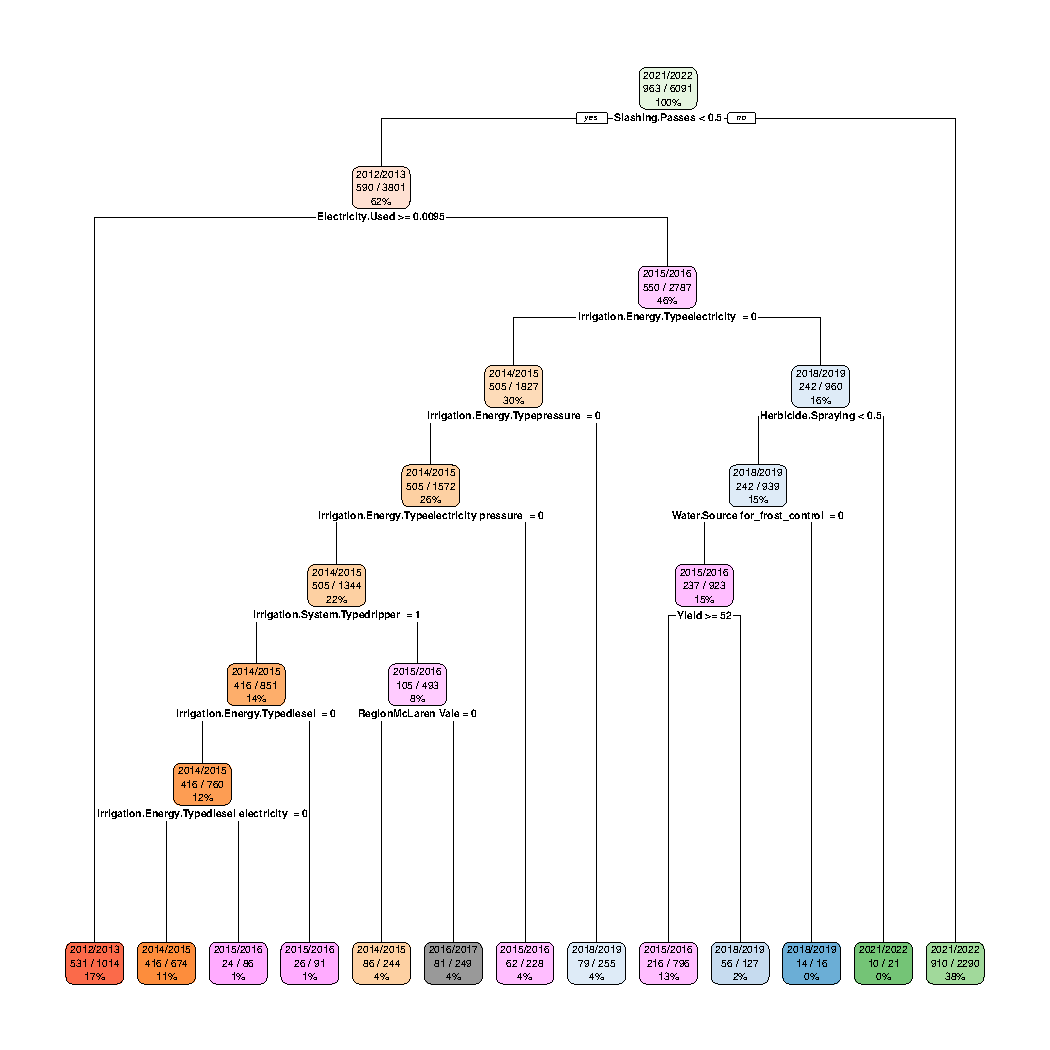
\includegraphics{year.pdf}}
  \caption{Decision tree predicting Year. Each node indicates the class predicted, and the proportion of elements agreeing with nodes partitioning, with the left direction indicating a yes to the nodes rule.}\label{fig:year_tree}
 \end{figure}
 
 \begin{figure}
  \resizebox{\textwidth}{!}{
  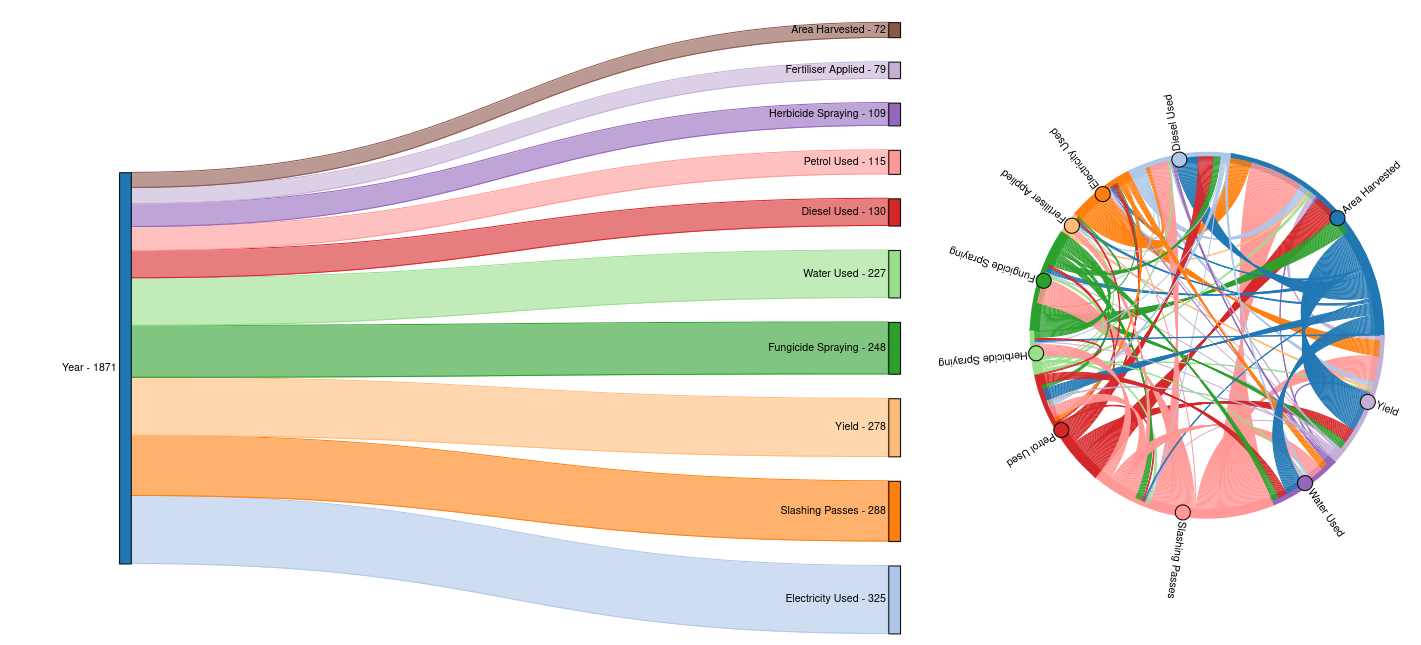
\includegraphics{year.png}}
  \caption{The left-hand side depicts the 10 most relative important variables in predicting Year using XGBoost as a measure of node occurrence, using a Sankey diagram. The right-hand side depicts the interrelated importance of the ten predictor variables using a chord diagram.}\label{fig:year_sankey}
 \end{figure}

 \subsection{Profit}

\begin{figure} 
  \resizebox{\textwidth}{!}{
  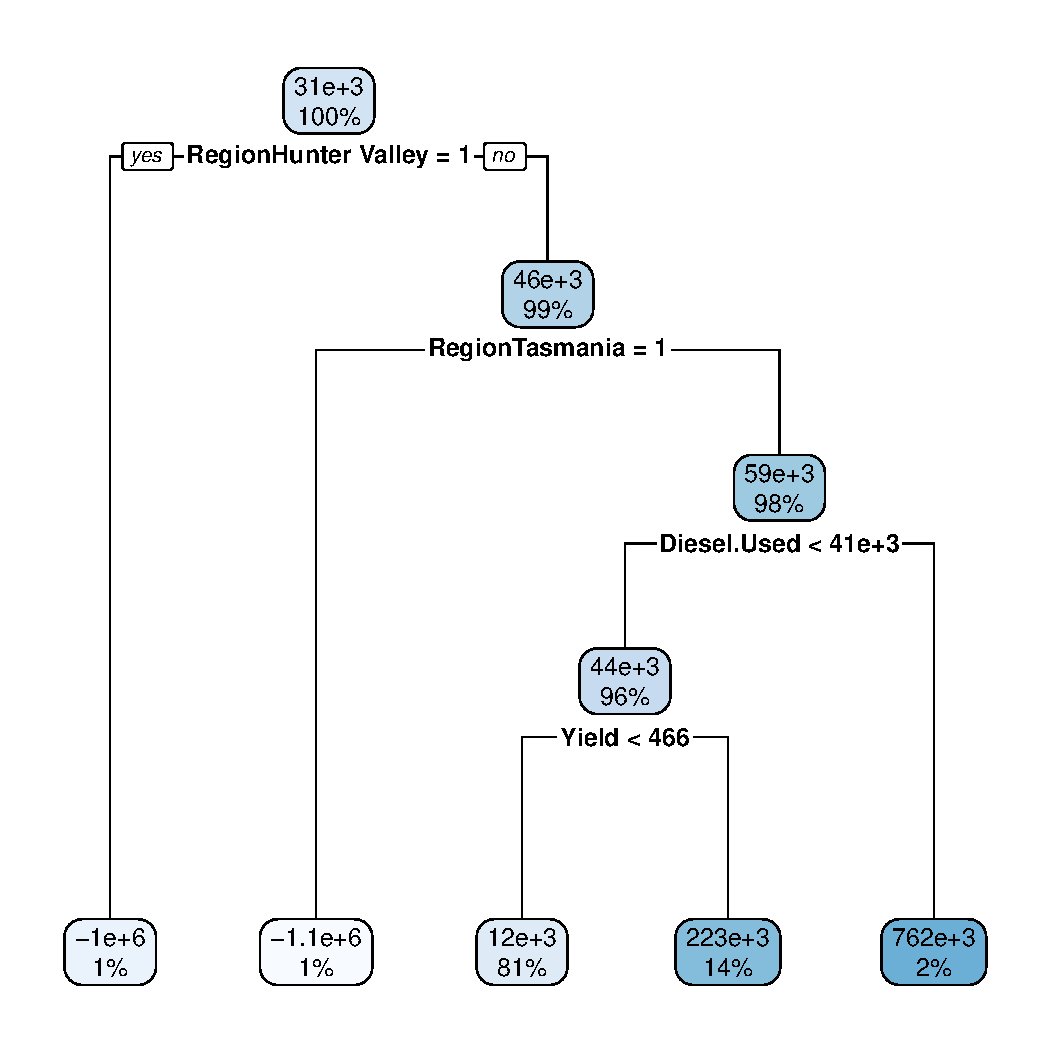
\includegraphics{profit.pdf}}
  \caption{Decision tree predicting revenue. Each node indicates the class predicted, and the proportion of elements agreeing with nodes partitioning, with the left direction indicating a yes to the nodes rule.}\label{fig:revenue_tree}
 \end{figure}
 
 \begin{figure}
  \resizebox{\textwidth}{!}{
  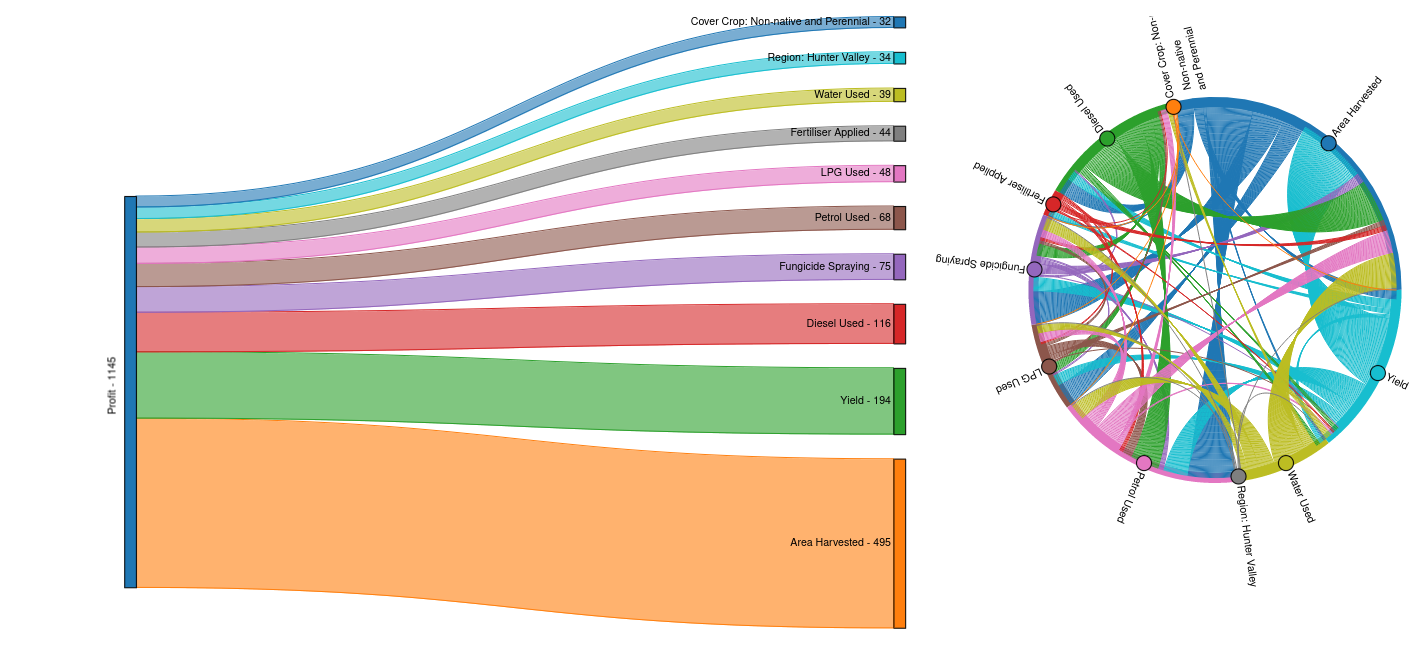
\includegraphics{profit.png}}
  \caption{The left-hand side depicts the 10 most relative important variables in predicting revenue using XGBoost as a measure of node occurrence, using a Sankey diagram. The right-hand side depicts the interrelated importance of the ten predictor variables using a chord diagram.}\label{fig:profit}
 \end{figure}

Predictions of profit perfomed poorly compared to operating cost and revenue with an average $R^2$ of 0.2535 and standard deviation of 0.3126. With the large standard deviation being indicative of how unstable the models created were.

\end{linenumbers}
 \end{document}
 
\endinput
